\documentclass[prd, nofootinbib, floatfix, 11pt,tightenlines,times]{article}

% latex W13report.tex; bibtex W13report; latex W13report; latex W13report; dvips W13report; ps2pdf W13report.ps ; gv W13report.pdf

\usepackage[paperwidth=8.5in,paperheight=11in,centering,margin=1in]{geometry}
\usepackage{amsmath}
\usepackage{amsbsy}
\usepackage{natbib}
\usepackage{rotating}
\input epsf
\usepackage{amsmath}
\usepackage{wasysym}
\usepackage{subfigure}
\usepackage{graphicx}
\usepackage{epsfig}
\usepackage{color}
%\usepackage{ulem}
%\usepackage{epstopdf}

\renewcommand{\thefootnote}{\fnsymbol{footnote}}

%\renewcommand{\baselinestretch}{0.98}
\usepackage{epsfig}
\usepackage{titletoc}

% HOW TO SET UP AN 8.5 x 11:
% http://www.pages.drexel.edu/~pyo22/students/latexRelated/latexTutorial.html
\topmargin -1.5cm        % read Lamport p.163
\oddsidemargin -0.04cm   % read Lamport p.163
\evensidemargin -0.04cm  % same as oddsidemargin but for left-hand pages
\textwidth 16.59cm
\textheight 21.94cm 
\parskip 7.2pt           % sets spacing between paragraphs
\parindent 0pt		     % sets leading space for paragraphs

\def\aap{{\it Astr.~Ap.}}     %Astronomy & Astrophysics%
\def\aaps{{\it A\&AS}}
\def\apj{{\it ApJ}}

\author{Andrew Becker, Simon Krughoff, Andrew Connolly, Russell Owen}
\title{Report on Late Winter2013 Production: Image Differencing}
\date{\today}

\begin{document}

\maketitle

Summary.

\clearpage
\tableofcontents
\clearpage

\section{Production Scope and Goals}

The focus of this production was to optimize and quantify the false
detection rate in the PSF--matched subtraction of a science image and
a reference image (referred to as the template image below).  We used
simulated images generated using ideal conditions, and with no
intrinsic variability in the sources.  The metric we optimized is the
number of false detections that are detected and measured on the image
difference.  As the input were simulated with no variability, any
detections found in the difference images are ``false positives''.  We
calculated several additional quality metrics during the image
subtraction process, and correlated them with the number of false
detections, as a means to predict the number of false detections we
may expect downstream from the image subtraction.  Once we found an
optimum configuration, we perturbed the solution along multiple
dimensions to understand how the false detection rate responded.  

\subsection{Algorithm and Background {\bf ANDYB}}

We outline the image subtraction process below.  We assume that science
image $S(x,y)$ can be modeled as a convolution of the template image
$T(x,y)$ by a PSF--matching kernel $K(u,v,x,y)$.  The images will have
different point spread functions (PSFs), which are the time--averaged
transfer functions of a point source through the Earth's atmosphere,
telescope optics, and into the silicon of the detector before being
read out.  The essence of image subtraction is to match the PSFs of
these two images so that they may be subtracted pixel by pixel.  We
further assume that the PSF--matching kernel may be decomposed using a
set of basis functions $K(u,v) = \sum_i a_i K_i(u,v)$, where the
coefficients in front of each basis are determined through:
%
\begin{eqnarray}
C_i & \equiv & (K_i \otimes T) \\ \nonumber
b_{i}  & = & \sum_{x,y} {{C_i(x,y) S(x,y)}\over{\sigma^2(x,y)}}   \nonumber \\ 
M_{ij} & = & \sum_{x,y} {{C_i(x,y) C_j(x,y)}\over{\sigma^2(x,y)}}  \nonumber \\ 
a_{i}  & = & M^{-1}_{ij} b_{j} \nonumber 
\label{eq-soln}
\end{eqnarray}
where $\sigma^2(x,y)$ is the per--pixel variance stored in the {\tt
  variance} plane of each LSST {\tt exposure}.  To generate a
spatially varying model for the kernel, we assume that the relative
weights of the basis functions $a_i$ themselves vary spatially,
i.e. $K(u,v,x,y) = \sum_i a_i(x,y) K_i(u,v)$.  We also assume that
there is a differential background between the two images $b(x,y)$
that may be fit for using a low--order Chebyshev polynomial.  The
image difference is then calculated through $D(x,y) = S(x,y) - T(x,y)
\otimes K(u,v,x,y) - b(x,y)$.

The basis functions themselves $K_i(u,v)$ are a degree of freedom in
this problem.  The original implementations \citep{Alard98,Alard00}
used a set of 3 Gaussians (represented by our {\tt Config} variable
nGauss), each with a different sigma (sigGauss), and each modified by
a Laguerre polynomial to a given order (degGauss).  Subsequent studies
\citep[e.g.][]{2007AN....328...16I} have suggested that a constant
ratio be maintained between the different Gaussian widths, such that
$\sigma_{i+1} = \beta \times \sigma_{i}$.  We use the value $\beta =
2.0$ for this production.  We set the overall scale for sigma by
noting that, under the assumption that the PSFs of the images are
Gaussian ($\sigma_S$ for the science image and $\sigma_T$ for the
template image), the sigma of the matching kernel should be simply
$\sigma_K^2 = \sigma_S^2 - \sigma_T^2$.  We use this width for the
central Gaussian in the basis sequences where we use more than one
Gaussian, or the sole Gaussian in the sequences when we use only one.

Detection on the difference image occurs through correlation of
$D(x,y)$ with the science image's PSF, yielding optimally filtered
detection image $D'(x,y) = D(x,y) \circ PSF_S(x,y,u,v)$ where $\circ$
denotes correlation.  The values of the pixels in $D'(x,y)$ provide a
maximum likelihood estimate of there being a point source at that
position.  Detection occurs by simply finding pixels that are more
than N sigma above the variance.  

In this production, we investigated two orders of operations for the
optimal filtering by the PSF.  In the first method, called
prefiltering, we PSF--match the template image to a pre--filtered
science image:
\begin{eqnarray}
D_{Pre}(x,y) & = & S(x,y) \circ PSF_S(x,y,u,v) - T(x,y) \otimes K(u,v,x,y) \nonumber \\ 
D'_{Pre}(x,y) & = & D_{Pre}(x,y). \nonumber 
\end{eqnarray}
By pre--smoothing the image that we are matching the template to --
$S(x,y) \circ PSF_S(x,y,u,v)$ -- we more frequently avoid the case
of PSF--matching {\it deconvolution}, where the FWHM of $T$ is
narrower than $S$.  This pre--filtering increases the FWHM of the
image by $\sqrt{2}$.  The PSF matching kernels will need to be
correspondingly larger to account for the larger PSFs.  We are able to
run detection directly on this image.

In the second, which is the classical postfiltering implementation of
the technique, we create a difference image that is then
post--filtered with the PSF for detection:
\begin{eqnarray}
D_{Post}(x,y) & = & S(x,y) - T(x,y) \otimes K(u,v,x,y) \nonumber \\ 
D'_{Post}(x,y) & = & D_{Post}(x,y) \circ PSF_S(x,y,u,v).  \nonumber 
\end{eqnarray}

%One complication is that measurement on $D'_{Pre}$ is necessarily
%different than on $D'_{Post}$.

\section{Input Data {\bf ANDYC}}

These algorithms were run on 3 visits, with seeings 0.6'' (visit
6866601), 0.88'' (visit 6866602), and 1.2'' (visit 6866603).  These
visits were simulated with {\bf DETAIL}.  All 9 sensors of the central
raft were simulated, for a total of 27 difference images per
configuration to use in our comparative analysis.

A template image was generated by {\bf DETAIL}.  The template has a
seeing of 0.88''.  This means that the matching of the template image
with visit 6866601 will yield a template {\it deconvolution} in the
postfilter configuration.  Matching of the template image with visit
6866602 also yields a mild deconvolution (the images were generated to
have the same seeing) for 5/9 sensors.  The matching of the template
with visit 6866603 with postfiltering, and of all visits with
prefiltering, yields a convolution (smoothing) of the image.

\section{Work Performed}

Tasks that were completed in the run--up to production include:
implementing prefiltering for image subtraction (ticket \#2551);
implementing source selection for image subtraction (\#2554, \#2596);
implementing measurement for difference image source (DiaSource)
characterization (\#2595); implementing RegisterTask for
image--to--image registration (\#2562, \#2650); defining and
implementing metrics for testing ip\_diffim (\#2636); designing a tool
to scrape metadata from data repositories (\#2640); and implementing
flux measurement for spatially filtered sources (\#2754).

Below we describe in detail the overall pipeline that was established
as the results of these tasks.  We follow with in--depth analysis of
implemented algorithms that are central to this production.

\subsection{Pipeline Implementation {\bf ANDYB}}

At the beginning of the pipeline, we have the science image $S(x,y)$
as a {\tt calexp} instance as an input.  The bounding box of the
science image, in celestial coordinates, was used to query the coadd
repository to return the coadd patches that overlap the image.
However, because of difficulties in fitting absolute astrometry to the
images (Section~\ref{subsec-astrom}), we instead took the approach of
directly using the {\tt calexp} of the deep visit as the reference
visit (as opposed to taking this deep {\tt calexp} and turning it into
a coadd).

Next, we used the DiaCatalogSourceSelector to query the ImSim
reference catalog for appropriate sources to use for PSF matching.
This selector allows the user to specify the brightness and color
range of the objects, toggle star or galaxy selection, and to include
variable objects or not.  We selected a fraction (1/5) of these
objects to serve as a control sample, in order to assess the
effectiveness of $K(u,v,x,y)$ to subtract objects that were {\it not}
used in the least squares fit.

The reference and science {\tt calexps} were then astrometrically
registered to each other, with the resampling operations happening on
the reference visit as it has the larger signal--to--noise (S/N).
Object--to--object matching, done using the source list above
cross--matched with a source list extracted from the coadd, was used
to provide a relative transformation between the two images.
RegisterTask was used to do the astrometric resampling.  The resulting
warped reference image was what we use as the template image $T(x,y)$.
The residuals of the object--to--object match were persisted as part
of the debugging infrastructure.  We assumed that the background
subtraction on the input {\tt calexps} removed the high order features
in the backgrounds; therefore we simultaneously fit for a 1st--order
spatially varying differential background $b(x,y)$ along with the
kernel coefficients.

Images $S(x,y)$ (optionally pre-filtered with $PSF_S(x,y,u,v)$) and
$T(x,y)$ were sent to ImagePsfMatchTask, whose purpose is to fit for
$K(u,v,x,y)$ and to produce $D(x,y)$.  The first step is to use the
PSF Gaussian sigmas to define the {\it sizes} of the Gaussians shapes
in $K_i(u,v)$.  As mentioned above, the main width was chosen to be
$\sqrt{\sigma_S^2 - \sigma_T^2}$.  We investigated variations on the
configuration where we used one Gaussian with the above width, and
where we used three Gaussians, the central of which has this width and
the others are a factor of $\beta = 2.0$ smaller and larger.  We
modified each of the Gaussians by a set of Laguerre polynomials of a
given order.  The smallest Gaussian was modified to the highest order,
with the others modified by order//2.  Figure~\ref{basis} provides an
example basis set with this configuration.  The total number of shapes
in each basis were: $\sum_i^{\rm nGauss} ({\rm degGauss}_i+1)\times({\rm
  degGauss}_i+2)/2$ \footnote{ A notable exception to this algorithm
  is found in the case where $\sigma_T > \sigma_S$, i.e. a sharpening
  must be done to the template to match it to the science image.  This
  is the case of deconvolution.  A theoretical prescription for basis
  design in this case is given in \cite{0266-5611-26-8-085002}.  In
  this algorithm, nGauss is {\it always} fixed to value 3, and
  degGauss is always fixed to 3.  The widths of the Gaussians are
  determined through the algorithm specified in
  \cite{0266-5611-26-8-085002}, using as inputs the sequence of
  Gaussians that we would have used to match a Gaussian of width
  $\sigma_S$ to $\sigma_T$ (i.e. as if we would have convolved the
  science image and not the template image).  There are a variety of
  reasons that actually operating on the science image is undesirable,
  including: the science image is lower S/N than the template; the
  science image is likely to have masked defects, including cosmic
  rays and bad pixels, whose reach would be expanded due to the
  convolution; unmasked features such as faint cosmic rays are more
  likely to look PSF--like after convolution (cosmic rays will likely
  have been sigma clipped out of the coadd).  However, it is not clear
  that deconvolving the template image is in principle any better.  A
  far better option, which we explore here, is to pre--filter the
  science image, which will in the vast majority cases provide a
  larger PSF (larger by $\sqrt{2}$) to match the template to.  This is
  the case for v6866601 in this study, where the postfiltered analysis
  yields deconvolution of the template, while the prefiltered analysis
  does not.  }.
%
The dimensions of the PSF matching kernel were
chosen to be 6 times the largest Gaussian width, with a minimum
kernelSize of 21x21 pixels.  For kernels that are significantly
smaller than this, the Gaussians have significant (non--zero) power at
the kernel boundaries, leading to square systematic artifacts at the
scale of the kernel in the difference images.


\begin{figure}
\centering{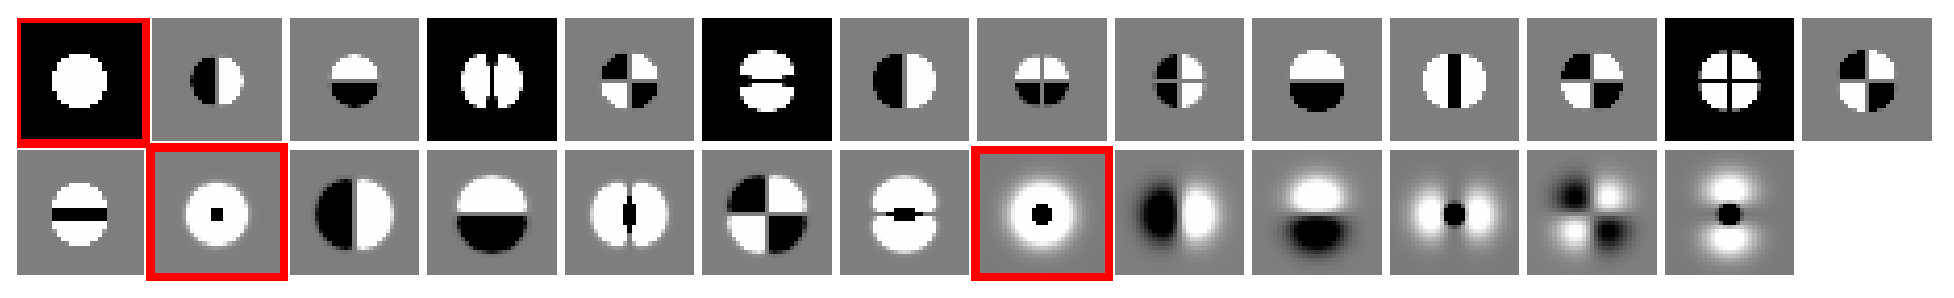
\includegraphics[width=0.8\textwidth]{figures/basis3.eps}}
\caption{Example basis set with nGauss=3 (highlighted in red),
  sigGauss=(0.5 sig, 1.0 sig, 2.0 sig), and degGauss=(4,2,2).}
\label{basis}
\end{figure}

For each source $j$ returned by DiaCatalogSourceSelector, we created a
{\tt KernelCandidate} instance, which holds substamps of $T_j(x,y)$
and $S_j(x,y)$ centered on the source.  These were used to fit for a
local solution $K(u,v)$; the ensemble of local solutions at each
source's $x,y$ was used to fit for the full spatial solution
$K(u,v,x,y)$.  We emphasize that the dimensions of the substamps are
important.  Note from equation~\ref{eq-soln} that the coefficients
$a_i$ are derived from a convolution of the template substamp with the
kernel basis functions $K_i$.  This convolution means that
kernelSize//2 pixels along each substamp edge are rendered unusable.
To maintain a significant number of pixels in $C_i$, we set the {\tt
  KernelCandidate} dimensions to be twice that of the kernel (i.e. the
number of pixels remaining in $C_i$ is equal to the number of pixels
in the kernel, which is fewer than the number of bases $i$).  For each
{\tt KernelCandidate}, we solved for $K(u,v)$ and create a local
difference image $D_j(x,y)$.  We evaluated several statistics on this
local difference image, normalized by the square root of its variance,
which puts the pixels in units of sigma.  We measured the mean sigma,
the RMS of this distribution, the $\chi^2$ of these pixels normalized
by the degrees of freedom (number of pixels in $D_j(x,y)$ minus the
number of kernel bases), and the mean squared error.  These are
referred to as the LOCAL kernel metrics, and reflect how appropriate
the chosen kernel basis is.

The ensemble of {\tt KernelCandidates} was then used to constrain a
spatial model of the kernel $K(u,v,x,y)$.  This was done using the
{\tt SpatialCellSet} formalism, whereby the {\tt KernelCandidates} are
distributed across the image in a grid of {\tt SpatialCells}.  This
formalism attempts to distribute constraints on the spatial model
evenly across the image.  At most 3 {\tt KernelCandidates} per {\tt
  SpatialCell} were input to the spatial kernel fit.  For the spatial
kernel model, we assumed that each of the kernel coefficients $a_i$
may be represented by a $N^{th}$ order 2--dimensional Chebyshev.
Normally, we would perform sigma--clipping iterations on candidates
having bad residuals after spatial modeling.  However in this
production we expect that all objects should fit, so we performed no
sigma clipping.  Having generated the full spatial solution
$K(u,v,x,y) = \sum_i a_i(x,y) K_i(u,v)$, we evaluated the kernel
solution at the position of each {\tt KernelCandidate}, created a
difference image using this kernel, and recalculated the metrics
defined above.  These are referred to as the SPATIAL kernel metrics.
Importantly, we also interpolated this solution to the positions of
the control sample, which were explicitly {\it not} used in the
spatial fit, and evaluate these same metrics.  The differences between
the {\tt KernelCandidate} LOCAL and SPATIAL metrics, as well as the
values of the SPATIAL metrics for the control sample, reflect the
appropriateness of the spatial model and our ability to interpolate
and extrapolate to the full extent of the images.  We used the Mean
Square Error (MSE) of the control sample to example the tradeoff
between bias and variance in the spatial interpolation.

We next ran the SourceDetectionTask on the difference image, using a
``polarity'' of {\it both} to search for both positive and negative
deviations.  We initially used a nominal detection threshold of 5
sigma.  In the case of pre--filtering, we detected on the difference
image directly.  In post--filtering, we correlated the difference
image with its PSF (by design, the same as the PSF of $S$) before
detection.  All else being equal, the images immediately preceding the
detection step ($D'$) should be {\it exactly} the same.  However,
differences in the shapes and sizes of the PSF--matching kernels used
in the two cases may cause systematic differences in the images.
Detections were merged using a grow radius of 2 pixels.

Finally, we ran DipoleMeasurementTask on the detections to create {\tt
  DiaSources}.  DipoleMeasurementTask is an extension of
SourceMeasurementTask that includes specific dipole measurement
algorithms.  Measurement was necessarily different in the
pre--filtered and post--filtered data.  In particular, in
post--filtering, detection happens on the filtered maximum likelihood
image and measurement on the associated pixels in the unfiltered
difference image.  In pre--filtering, the latter image does not exist,
and thus detection and measurement happen on the same image.  This
restricts the types of measurements that may be made on the sources.
For example, the PSF flux is merely the fitted amplitude of the peak
in the image, and the PSF centroid its center.  While these
measurements were straightforward to implement, additional work needs
to be done on how to implement the remainder of the measurement suite
on post--filtered data.

All {\tt DiaSources} were associated with the {\tt calexp's} sources
and with the reference catalog, with a permissive matching radius of
3''.  {\tt DiaSources} that matched with sources may be true residuals
around stars {\it or} true false positives that are also found in the
{\tt calexp} SourceDetectionTask.  For this reason, we used the
associations with the reference catalog objects as the assessment if a
given {\tt DiaSource} matched with an input object or whether it was
an orphan (e.g. a statistical fluctuation in the background).  In
addition, all {\tt KernelCandidates} were persisted with the above
{\tt LOCAL} and {\tt SPATIAL} metrics.  Repositories were accessed
with a specially written RepositoryIterator that aggregates {\tt
  KernelCandidates} from a given source across multiple output
repositories.  Finally, the {\tt DiaSource} lists for all production
repositories were compared to find the configurations that yielded the
lowest numbers of false detections.

\subsection{Improvements to Measurement {\bf RUSS}}

Compare the measured S/N of the DiaSources with the detection threshold.

\subsection{KernelCandidate Statistics}

\subsubsection{Mean Squared Error {\bf SIMON}}

In order to investigate the bias--variance trade--off in the overall
fit, we calculate the MSE of each {\tt KernelCandidate's} difference
image derived from the evaluation of the spatial model at that
location.  We define the bias as $\left| data - model \right|$, the
variance as $\left| (data - model)^2 \right|$, and the MSE as {\tt
  bias$^2$ + variance}.  In this context, the bias is the mean of the
difference image, and the variance is the mean square of the
difference image.  In both cases, we normalize by the square root of
the variance so that pixels are in units of sigma.

\subsubsection{Reduced $\chi^2$ {\bf SIMON}}

\subsubsection{Control Sample {\bf SIMON}}

\section{Production Runs {\bf ANDYB}}

We ran several pre--productions to tune the following aspects of the
pipeline: the dimensions of the kernels and {\tt KernelCandidates};
the widths of the Gaussians (sigGauss) based on the FWHM of the input
images; and the scaling of the Gaussians ($\beta$) in the basis
sequence.  Figure~\ref{fig_galleryBad} provides a rogue's gallery of
image subtraction failures encountered at this stage, each centered on
{\tt KernelCandidates}, and outlines reasons for each failure.
Figure~\ref{fig_galleryGood} provides a gallery showing what the
results from a successful image subtraction appeared like, for
postfiltering on the {\it top} and prefiltering on the {\it bottom}.

The main production runs included: an outer loop over the use of
pre--filtering or post--filtering for detection; variations of the
complexity of the Kernel basis, including the number of Gaussians
(nGauss = 1,3) and the degree of the modifying Laguerre polynomials
(degGauss = 1..6); and the spatial order of the Chebyshev polynomials
on $a_i(x,y)$ (spatialKernelOrder = 1..6).  The final production run
was labeled {\bf run10}, and data are available on the NCSA compute
cluster\footnote{/nfs/lsst8/becker/sparse\_diffim/production10\_sparse}.

Finally, we ran several post--productions focused on perturbing the
solutions that yielded the fewest numbers of DiaSources along specific
dimensions.  This included: the RMS of the WCS solution used by
RegisterTask; including a DC offset in the source positions prior to
RegisterTask, to determine the ability of the kernel basis to
accommodate astrometric misregistration; the size of the {\tt
  SpatialCells} used in the spatial interpolation, which effectively
regulates the numbers of constraints that go into the spatial fit; and
modifying the detection thresholds to determine how the number of
false detections scales with threshold.


\section{Results: False Detection Rate}

\subsection{Theoretical {\bf ANDYC}}

\subsection{Empirical {\bf ANDYB}}

After running an ensemble of 144 pipeline configurations, we
aggregated the numbers of false detections.  We report the results for
the each of the 3 visits, and for pre-- and postfiltering for
detection.  We cut on {\tt flags.pixel.edge} to remove spurious
detections on the immediate border of the image; other than that we do
no other cuts other than requiring that the {\tt centroid.sdss} is
finite.  We separated the DiaSources that match with the reference
catalog (3'' matching radius) from those that don't (referred to as
orphans) to investigate the origins of the detections.  We found no
significant correlation of false detections with sensor within the
raft; therefore we report the aggregate results for all 9 sensors in
the analyses that follow.

A set of ``heat maps'' are presented in Figure~\ref{fp_heatmap}, that
demonstrate the total number of detections across all 9 sensors as a
function of the config parameters spatialKernelOrder and degGauss, for
nGauss = 3.  Qualitatively, these heat maps indicate that a Chebyshev
spatial order greater than 3 is required for all data.  In addition,
with the exception of the deconvolution case (visit 6866601 and
prefilter=False), the Gaussians need to be modified by Laguerre
polynomials of order 4 or higher.  The minimum of these detection maps
are found using the configs of highest complexity, with a very flat
slope in the number of false detections beyond spatialKernelOrder$>$3
and degGauss$>$3.  There is not much evidence for an upturn in the
numbers of false detections, meaning we have likely not reached the
case of overfitting using these configs.

The numbers of false detections in each best case are given in
Table~\ref{tab-bestfp10}.  We undertook a manual inspection of all
difference images to associate the DiaSources with Sources in the
images, and also use a 3'' association with the input source catalog
to define matches and orphans.  Associations are listed in the
N$_{Match}$ column of Table~\ref{tab-bestfp10}, with the unmatched
false positives in the N$_{Orphan}$ column.  The former are likely to
come from systematics in the subtractions of stars, while the latter
would be due to fluctuations in the background.  We note 2 effects
that will impact N$_{Match}$.  The first is that, with a 3'' matching
radius, 4\% of random fluctuations will by--chance associate with a
Source.  Assuming that N$_{Orphan}$ represents 96\% of the background
fluctuation population, we estimate the number of fluctuations from
that same population that would have associated with Sources as
N$_{Random}$.  Finally, we count all matches that occur within 100
pixels of the image boundary, where we might expect the spatial
extrapolation to yield systematic residuals, as N$_{D<100}$.  To the
extent that (N$_{Random}$ + N$_{D<100}$) $<$ N$_{Match}$, we have a
small residual set of systematic false detections in our imaging
ensemble.  Aside from the deconvolution run, this is at the level of
10 total false detections over 9 sensors in 5 production runs, or 1
every 4--5 images.

We also list the ratio of negatively detected to positively detected
DiaSources.  That this ratio is significantly greater than 1.0 in most
cases suggests that there is an over-subtraction of the background in
the process, which biases this ratio (see Section~\ref{sec-bg}).  The
optimal configurations yielding these false detection rates are given
in Table~\ref{tab-bestconfig10}.

We have examined the distribution of these false detections across the
image, and find no significant overdensities near the borders of the
images, which would be expected in cases of under or over--fitting of
the various spatial models (astrometry, backgrounds, PSF--matching
kernels).  Figure~\ref{edgedist} provides the distribution of
distances from the edge of the sensor for all false detections in {\it
  blue}, with a random sample of points in the image given in {\it
  green}.  Uncertainties are plotted using the square root of the
number of points in each bin, and the histograms are normalized to
provide a probability density.  The takeaway is that we find no
significant correlation of false detections with the boundaries of the
fitting functions.

\section{Results: False Detection Dependencies}

After finding the configurations that yielded the minimal numbers of
false detections, we then perturbed the solutions to examine how the
numbers of false detections scaled with different effects.  This
included, in order of importance for this production: the difference
image detection threshold; the number of {\tt KernelCandidates} going
into the spatial model; and astrometric registration errors.  We also
undertook a theoretical analysis of the number of false detections
expected in a 4k x 4k image as a function of detection threshold, and
examine the requirements this sets on our ability to model the
variance and backgrounds in the images.  We compare the empirical
variation of false detections with detection threshold in our data,
and show that our results are consistent with this, indicating that we
reached the systematic floor in these data.

\subsection{Detection Threshold {\bf SIMON}}

Section \ref{sec-analyticfp} discusses the theoretical foundation 
that sets the floor on the number of false positives we expect from a 
pure Gaussian random field.  The number of false positives is a strong
function of the seeing and and the confidence level of the detection.  
By comparing the empirical false positive rate to the analytic predictions
we can quantify how close we are getting to the theoretical floor in these
data.  Because the number of false positives is such a strong function of
detection threshold, misestimation of the signal to noise of the detections
has a large impact on how many false positives are observed.  The Figures
\ref{fig-fpthresh1}, \ref{fig-fpthresh2}, and \ref{fig-fpthresh3} show the 
effect of misestimating the noise in the detections for each of three different
seeing values (0.6\", 0.88\", 1.2\" respectively).


To estimate the numbers of false detections we would expect in a
$4000\times4072$ pixel science image with a given FWHM in pixels, we
do the following.  The theoretical expectations for the number of
false detections due to random Gaussian fluctuations is outlined in
\cite{Kaiser-PointSources}.

\subsection{Number of KernelCandidates {\bf ANDYB}}

We effectively decreased the numbers of {\tt KernelCandidates} in the
spatial solution by increasing the size of {\tt SpatialCells} used to
model the solution, while keeping the number of objects used from each
cell the same.  We increased this from the default size of 128 pixels
to (256, 384, 512, 640) pixels.  We tracked the numbers of false
detections, and the number of used {\tt KernelCandidates}, and these
curves are displayed in Figure~\ref{cellsize}.  The {\it left} panel
shows the numbers of false detections, while on the {\it right} the
numbers of {\tt KernelCandidates} used, summed across all 9 sensors.

We note that in the prefiltered data the numbers of false detections
are not strongly dependent on the number of constraints on the spatial
solution.  For visits v6866601 and v6866603 this number is even seen
to decrease with decreasing {\tt KernelCandidates}.  This suggests
that in prefiltering there is not a significant different in quality
of fit when using $\sim$600 vs. $\sim$300 {\tt KernelCandidates} per
sensor.  The overall fit is demonstrably worse when using only
$\sim$100 constraints on the model (cell size = 640).  The indication
is that 300 constraints on the spatial model (which has 28, 28, and 21
terms per basis for visits v6866601, v6866602, and v6866603
respectively) appears sufficient in the case of prefiltering.

In the case of postfiltering, aside from the deconvolution case, the
number of false detections continually increases as the number of {\tt
  KernelCandidates} decreases.  This indicates that the best mode to
operate in when postfiltering is to maximize the number of constraints
on the model.

\subsection{Registration Errors {\bf ANDYB}}

We implemented two simple perturbations of the inputs to the
image--to--image RegisterTask: we first added a random offset to each
object's (x,y)-coordinates, with an amplitude that was specified in
the Config and multiplied by a random number pulled from a normal
distribution; and we added a DC offset to the coordinates at an
amplitude specified in the Config.  These offsets, added to the Source
coordinates, will cause misalignments of the objects in the registered
images, as the registration is done assuming the specified positions
are correct.  In this way we are able to investigate how random
uncertainties and bulk astrometric offsets impact the false positive
rate.  We explicitly do {\it not} investigate spatial variation in
these offsets, using for example a pincushion distortion.  We
anticipate that this latter effect will be most important for spatial
interpolation and extrapolation of the matching kernel, yielding a
dipole residual field associated with the distortion.  However, we
start with the basics here to investigate the individual terms in such
misalignments.

\subsubsection{Coordinate RMS {\bf ANDYB}}

We perturbed the coordinates of each template Source that was input to
RegisterTask with amplitudes of (0.025, 0.05, 0.075, 0.1, 0.125, 0.15,
0.175, 0.2, 0.3, 0.4, 0.5, 1.0, 1.5, 2.0, 2.5, 3.0, 3.5, 4.0) pixels,
and to randomize the effects we multiplied each offset by a number
pulled from a normal (0,1) distribution.  The output RMS reported by
RegisterTask was noted to track these offsets.  

Figure~\ref{wcsrms} shows how the numbers of false positives scales
with this RMS.  Note that the distribution is very flat out to 1.0
pixel (0.2'') for all images except for the deconvolution
configuration.  The number of false positives doubles after an RMS of
1.5--2.0''.  This test indicates that, for this very simplified case,
random astrometric uncertainties do not strongly impact the difference
image quality.  This may change with more realistic distributions of
stellar brightnesses, if individual objects pull the fit more than
others due to inverse variance weighting.  In this solution, with the
stars having the same brightness, no single random offset is likely to
drive the fit.

\subsubsection{Coordinate Offsets {\bf ANDYB}}

We offset the coordinates of each template Source that was input to
RegisterTask with amplitudes of (0.025, 0.05, 0.075, 0.1, 0.125, 0.15,
0.175, 0.2, 0.3, 0.4, 0.5, 1.0, 1.5, 2.0, 2.5, 3.0, 3.5, 4.0) pixels.
Post--registration, this will offset the positions of sources in the
two images by the desired amount.

Figure~\ref{wcsshift} shows how the numbers of false positives scales
with this shift.  Surprisingly, the distribution is very flat out to
nearly 1.0 pixels (0.2'') for all images except for the deconvolution
configuration.  The number of false positives doubles after a shift of
1.5''.  This test indicates that, for this very simplified case, bulk
astrometric offsets of the degree expected from nightly processing
should not drive the false positive rate.  

Figure~\ref{kernel_offsets} demonstrates the ability of the
PSF--matching kernel to redistribute flux to account for bulk
astrometric misalignments.  Since these offsets are common--mode
amongst all {\tt KernelCandidates}, the basis shapes themselves drive
the pipeline's ability to compensate for them.  Having a Gaussian
function whose sigma is commensurate with the amplitude of the offset
enables the software to place significant power in this basis term.  We
expect that, if these misalignments are a vector field, the ability of
the spatial kernel model to account for the spatial variation of the
misregistration will begin to drive the solution.  The take--away
from this analysis is that the PSF--matching basis appears flexible
enough to account for, individually, random scatter and bulk offsets
in the WCS solution.  This narrows the focus down to understanding how
spatial variation in the WCS may drive the difference image quality,
and what requirements need to be put both on the kernel basis and its
spatial variation.


\subsection{Background Subtraction {\bf SIMON} \label{sec-bg}}

\subsection{Variance Misestimation {\bf ANDYB/SIMON}}

{\bf good point: note that the curves nfp vs. threshold are
  correlated, its a cumulative distribution}.

Because these images will have gone through multiple convolutions
before reaching the detection stage, it is expected that the
propagated per-pixel variance will not provide an exact representation
of the empirical variance in the image planes \citep{Price-Stacking}.
Because the astrometric resampling uses a warping kernel that is
designed to preserve the noise properties of the images, we expect
that the kernel convolution and PSF--filtering will be the largest
sources of error.

To quantify these errors, we first compared the empirical variance in
the image planes with the level tracked by the variance planes.  We
calculated the ratio of the interquartile range of unmasked pixels in
the image plane, multiplied by 0.741 and then squared, with the median
of unmasked pixels from the variance plane.  The former represents the
empirical variance, while the latter the propagated variance.  We
investigate their ratio (empirical/propagated) at 2 stages in the
processing: after creation of the difference image (image $D$), and
immediately preceding detection (image $D'$).  Recall that for
prefiltering, $D = D'$.  These results are summarized in
Table~\ref{tab-variance1}.  For prefiltering, we find that the
variance plane typically underestimates the true variance by $1\%$ for
all visits.  When using postfiltering, the deconvolution visit
v6866601 yields a similar underestimate in the difference image, but
for the other two visits the variance is tracked to better than 1\%,
with a small RMS.  However, when postfiltering with the PSF, the
variance becomes {\it overestimated} by nearly a factor of two for
deconvolution visit v6866601, and {\it underestimated} by $4-5\%$ for
the other visits.

We further investigate the variance properties of the images that are
input to the detection stage, i.e. the difference image itself in the
case of prefiltering, and the difference image correlated with its PSF
in postfiltering.  These results are summarized in
Table~\ref{tab-variance2}.  We find that, empirically, the images have
very similar noise properties at the detection stage, with the
deconvolution visit having larger variance by $1\%$ but the other
visits having essentially equal noise properties, with a bias towards
the postfiltered data having slightly higher variance (while the RMS
is small, all values are greater than 1.0).  The medians of the
variance planes tell a different story though.  For the deconvolution
visit, the median per--pixel variance is $70\%$ higher.  While this
will suppress the detections of false positives, it will also
significantly suppress the detection efficiency for true variability.
For the other visits, the prefiltered per--pixel variance is
relatively {\it higher} by $3-4\%$.  This will decrease the
sensitivity of the prefiltered data to false positives; as shown
above, the rate is indeed smaller using the prefiltering pipeline.
This analysis demonstrates that this is primarily due to an {\it
  underestimate} of the per--pixel variance in the postfilter
processing: while the prefiltered variance is a 1\% underestimate, the
postfiltered variance is a 5\% underestimate.  As outlined by
\cite{Price-Stacking}, this may be due to differences in pixel
covariance when undergoing multiple convolutions, which are not
currently tracked.  We have not yet definitively demonstrated that
this is the case here.

For completeness, we note the median differences in the image plane at
the time of detection are 3--4 counts (or 0.2 sigma relative to the
empirical variance) for v6866601, 0.2 counts (0.02 sigma) for
v6866602, and less than 0.1 counts (0.01 sigma) for v6866603.

\section{Results: Computational Performance}

For this production, the understanding of the algorithm and
optimization of the false detection rates took priority over
optimizing the computational performance of the algorithms.  In
particular, debugging hooks were implemented and workarounds of
problems were devised with the focus on understanding the core
PSF--matching algorithm.  Therefore there are several key ways in
which the production as--implemented will differ from how the code is
used in Nightly and Data Release Processing.  We outline these
differences below.

The first difference is that due to problems with the {\tt
  meas\_astrom} package, detailed in Section~\ref{subsec-astrom}, we
were unable to exercise the envisioned data flow where we query a
coadd repository for the template image.  Instead we used a single
deep {\tt calexp} as the template image.  The astrometric registration
of these images was trivial, as the images almost exactly overlap and
are exactly the same size.  Thus the timings of the {\tt
  imageDifference:register} task are {\it underestimates} of the
astrometric registration subtask computational performance.

Second, the core performance of the {\tt imageDifference:subtract}
task will be significantly impacted by debugging hooks that were put
in place specifically to generate the metrics being evaluated in this
production.  The core functionality, {\tt matchMaskedImages}, does the
convolution kernel fitting and actual convolution of the template
image, and will be least impacted by these add--ons.  The reported
timings of {\tt matchMaskedImages} are thus an {\it overestimate} of
the method's performance.

The reported {\tt imageDifference:detection} task performance is an
accurate representation of its computational requirements.  However,
the {\tt imageDifference:dipolemeasurement} task represents a
significant overestimate of the true dipole measurement requirements.
In particular, the PSF--flux dipole measurement is explicitly
sub--optimal, in that its centroid fitting algorithm is a 4--deep {\tt
  for} loop.

With these caveats, the timings of the {\tt imageDifference} subtasks
are presented in Table~\ref{tab-timings}.

\section{Conclusions}

We can reach near the theoretical limit for false detection rate in
these ideal data, something which has not been demonstrated for image
subtraction algorithms in the past.

Pre--filtering is clearly preferred when the traditional process would
lead to deconvolution, or sharpening, of the data.  When the standard
processing results in a convolution, or smoothing of the data,
pre--filtering provides fewer false detections.  As a trade--off, the
measurement of these false detections is not yet well defined.

\begin{itemize}

\item We find that the overall number of false detections is not
  strongly sensitive to bulk background misestimation
  (Figure~\ref{XXX});

\item However, the ratio of positive to negative false detections is
  strongly dependent on background fitting, with {\bf XXX}
  (Figure~\ref{XXX}).

\item Our empirical negative to positive false detection ratio is {\bf
  X.X}, indicating a bias in the background levels of {\bf X\%}.

\item At the 5--sigma detection threshold, for the range of seeings
  considered in this production, the theoretical numbers of false
  detections per 4k x 4k sensor numbers 10+.  This function is steep;
  by increasing the detection threshold to 5.X sigma this number may
  be lowered to less than 1 per sensor.

\item Due to the steepness of this function, the number of false
  detections is strongly dependent on the variance being correct, at
  the 5--sigma detection threshold.  When detecting at 5--sigma,
  having the variance underestimated by 1\% leads to an increase
  in false positives of {\bf XXX} (Figure~\ref{}).

\item An empirical computation of the variance from the image plane,
  compared to the median propagated variance in the variance plane,
  indicates that we consistently underestimate the variance by $1-2\%$
  (Table~\ref{tab-variance1}).  A proper tracking of covariance during
  the multiple image convolutions that occur may alleviate this
  problem.

\item When convolving to PSF--match, variance planes of postfiltered
  detection images have {\it lower} variance than their prefiltered
  counterparts by $2-3\%$ (Table~\ref{tab-variance2}).  These images
  have gone through one additional convolution compared to the
  prefiltered data.

\item When strongly deconvolving, the postfiltered variance is 70\%
  {\it higher} at the time of detection compared to the prefiltered
  data (Table~\ref{tab-variance2}).  This is consistent with the
  understanding that deconvolution increases high frequency noise in
  the images, and provides a {\it lower} detection efficiency in
  deconvolved data.  Prefiltering is clearly preferred in the case of
  significant deconvolution (v6866601; FWHM of 4.9 pixels matches to a
  FWHM of 3.5 pixels).

\item The postfilter pipeline can produce difference images with a
  minor deconvolution (v6866602; FWHM of 4.9 pixels matched to 4.9
  pixels) at a quality commensurate with a subtraction that uses a
  smoothing convolution (v6866603; FWHM of 4.9 pixels matched to 6.7
  pixels).

\item The false detection rate is seen to scale with detection
  threshold in a manner consistent with theory (Figure~\ref{}).

\item Several statistics that we are able to calculate at the time of
  image subtraction are shown to correlate strongly with the numbers
  of false detections, providing real--time quality estimates
  (Figures~\ref{}).

\item The numbers of false detections that associate with Sources is
  shown to correlate with the amount of smoothing that occurs in the
  PSF matching, in the sense that more smoothing leads to fewer false
  detections (Figure~\ref{}).  In this sense, there is a strong
  preference for running in prefiltered mode.

\item Measurements on prefiltered difference images contain less
  information than in postfiltered difference images, because the
  paradigm of detection on filtered data but measurement on the
  unfiltered data is broken.  Thus while we detect on average fewer
  false positives in prefiltered data, we are (so far) able to
  characterize them less well.  This trade--off is clearly something
  to explore in future work.

\end{itemize}

\section{Outstanding Issues}
We ran into several issues while doing this production that required work 
arounds.  In some cases we did not have the time to drill all the way down
to the root cause.  We itemize these issues here so that they may be addressed 
as part of the Summer 2013 work.


\subsection{Astrometric Registration \label{subsec-astrom}}
The original plan for this production was to use single deep exposures as 
templates.  This required that we treat the single exposures as coadds.  As 
such we warped the exposures to coadd patches for use in the image difference
task.  The register task is unable to solve a differential WCS if one of the images
has the CRPIX off the image.  This is the case for coadd patches.  To get around this
we resolved the coadd patches using a TAN-SIP solution and then used the register
task to solve for the differential WCS.  This worked fairly will part of the time 
yielding residuals in the 40-100 mas range.  The rest of the time the 
residual was more like 250 mas range.  This is an order of magnitude larger than expected.

We investigated potential causes of the large residuals.  To do this, we looked at the 
residuals for template solutions, science image solutions, and template to science calexp 
registration to attempt to isolate where the astrometry was being degraded.  The results are shown
in table \ref{tab-wcsrms}.  We show the results for the nine sensors in the best seeing visit.  

The solutions for the three steps that do not involve any warping show results consistent with 
the accuracy we expect to get.  We also see the expected trend that the deep exposures have 
smaller RMS than the solutions of the science images and the differential solution is dominated
by the RMS in the science image.  In four cases, the coadd to science solution did not fail
as catastrophically as in the other five, but the RMS is still a factor of several larger
than in the non-warped cases.

\subsection{Detection and Measurement on Negative Sources}
We see more negative false positives than positive false positives.  This drove an investigation 
into the symmetry of detection on positive/negative sources.  To do this we looked at the results 
of the image difference task and compared it to the same runs when the difference image was inverted
$differenceImage *= -1$ before measurement.  The results are as follows:
\begin{itemize}
\item The DIA source lists are always the same length.
\item Negative sources always have integer centroid pixel values where positive sources have fractional
pixel precision.
\item Some sources are have the edge bit set in one image or the other.  This leads to a difference in 
the number of false positives as we only consider those without the {\tt EDGE} flag set.
\end{itemize}

The suspicion is that the difference in precision of the centroid is linked to the difference in flags.
We have not had the time to chase this down completely, but plan on doing so in Summer 2013.


\section{Future Work}

We intend to research additional aspects of the problem going forward,
including:
\begin{itemize}
\item How the false detection rate varies with more realistic SEDs;
\item How the false detection rate varies with airmass;
\item How the system behaves with a realistic mix of stars and galaxies;
\item How the false detection rate looks in crowded fields;
\item How to perform measurement on pre--filtered difference images;
\end{itemize}

\clearpage
\bibliographystyle{apj}
\bibliography{refs}

\clearpage
\begin{table}
\centering
\begin{tabular}{clcccccc}
\hline
\multicolumn{8}{|c|}{Best Results: Production 10} \\
\hline
Visit    & Prefilter & Total False Detections &  N$_{Orphan}$ & N$_{Match}$ & N$_{Random}$ & N$_{D<100}$ & Nneg / Npos \\
\hline
v6866601 & True      & 70      &60         & 10 & 3     & 4   & 1.8 \\ 
         & False     & 143     &51         & 92 & 2     & 11  & 0.4 \\
v6866602 & True      & 42      &36         & 6  & 2     & 1   & 2.6 \\
         & False     & 53      &45         & 8  & 2     & 1   & 0.5 \\
v6866603 & True      & 23      &23         & 0  & 1     & 0   & 2.8 \\
         & False     & 36      &35         & 1  & 1     & 0   & 3.4 \\
\end{tabular}
\caption{Total number of {\tt DiaSources} detected at 5--sigma from
  all 9 sensors in raft 2,2, for the configurations that yielded the
  lowest number of false detections.  Matches are determined using a
  3'' match radius with the input reference catalog.  Objects with the
  {\tt EDGE} flag are ignored.  We list the number of background
  fluctuations that are expected to randomly associate with a Source
  N$_{Random}$, given the density of objects in the images and a 3''
  match radius, assuming that N$_{Orphan}$ represents 96\% of the
  total population of detections arriving from Gaussian fluctuations.
  We also list the number of false detections that are found within
  the outer 100 pixels of the image N$_{D<100}$.  The final column
  lists ratios of the number of negatively detected false detections
  to those with positive flux, a 5--sigma. \label{tab-bestfp10}}
\end{table}


\begin{table}
\centering
\begin{tabular}{clccc}
\hline
\multicolumn{5}{|c|}{Best Configs: Production 10} \\
\hline
Visit    & Prefilter & nGauss & degGauss & spatialOrder \\
\hline
v6866601 & True      & 3      & 6        & 6 \\
         & False     & 3      & 1        & 5 \\
v6866602 & True      & 3      & 6        & 6 \\
         & False     & 3      & 6        & 5 \\
v6866603 & True      & 3      & 5        & 5 \\
         & False     & 3      & 4        & 6 \\
\end{tabular}
\caption{Configurations that led to the best results listed in
  Table~\ref{tab-bestfp10}.  All post-production runs include
  perturbations about these configurations. \label{tab-bestconfig10}}
\end{table}

\clearpage

\begin{table}
\centering
\begin{tabular}{clccc}
\hline
\multicolumn{4}{|c|}{Variance Ratios: Empirical / Propagated} \\
\hline
Visit    & $D_{pre} = D'_{pre}$ & $D_{post}$ & $D'_{post}$ \\
\hline
v6866601 &$1.012 \pm 0.002$&$1.018 \pm 0.005$&$0.599 \pm 0.017$ \\
v6866602 &$1.010 \pm 0.002$&$1.007 \pm 0.001$&$1.046 \pm 0.002$ \\
v6866603 &$1.015 \pm 0.003$&$1.008 \pm 0.001$&$1.045 \pm 0.003$ \\
\end{tabular}
\caption{Ratio of the empirical variance in the difference images,
  calculated via (0.741 times the interquartile range)$^2$, to the
  median of the variance plane.  In all cases the variance plane
  represents an {\it underestimate} of the true variance in the
  images.  We report the mean and RMS across all sensors for the best
  configurations.  }
\label{tab-variance1}
\end{table}

\begin{table}
\centering
\begin{tabular}{ccc}
\hline
\multicolumn{3}{|c|}{Variance Ratios: $D'_{post} / D'_{pre}$} \\
\hline
Visit    & Empirical & Propagated \\
\hline
v6866601 & $1.011 \pm 0.016$    & $1.710 \pm 0.049$    \\
v6866602 & $1.001 \pm 0.001$    & $0.967 \pm 0.001$    \\
v6866603 & $1.002 \pm 0.001$    & $0.974 \pm 0.002$    \\
\end{tabular}
\caption{Ratios of the variance planes immediately before detection
  $D'$.  Ratios are in the sense of the variance of the postfiltered
  image divided by the variance of the prefiltered image.  The first
  column represents the ratios of the empirical variance, calculated
  via (0.741 times the interquartile range)$^2$.  The second column
  reports the ratios of the means of the propagated variance planes.
  We report the mean and RMS across all sensors for the best
  configurations.}
\label{tab-variance2}
\end{table}


\clearpage
\begin{table}
\centering
\begin{tabular}{|c|c|c|c|c|}
\hline
\multicolumn{5}{|c|}{WCS RMS in mas at various stages} \\
\hline
Sensor    & Deep & Science &  Deep to Science & Coadd to Science \\
\hline
R22:S00&21&29&19&382\\ 
R22:S10&13&22&22&389\\
R22:S20&7&18&21&375\\
R22:S01&13&25&21&86\\
R22:S11&6&17&20&81\\
R22:S21&8&19&20&382\\
R22:S02&8&17&20&178\\
R22:S12&9&20&20&78\\
R22:S22&7&21&21&389\\
\hline
\end{tabular}
\caption{We looked at the resulting RMS from WCS fitting on the deep exposure alone, the science exposure alone,
fitting the deep exposure to the science exposure, and fitting a warped coadd to the science exposure.  Fitting 
the coadd to the science exposure produces an order of magnitude more scatter in the fit than at any other point.\label{tab-wcsrms}}
\end{table}
\clearpage


\begin{figure}
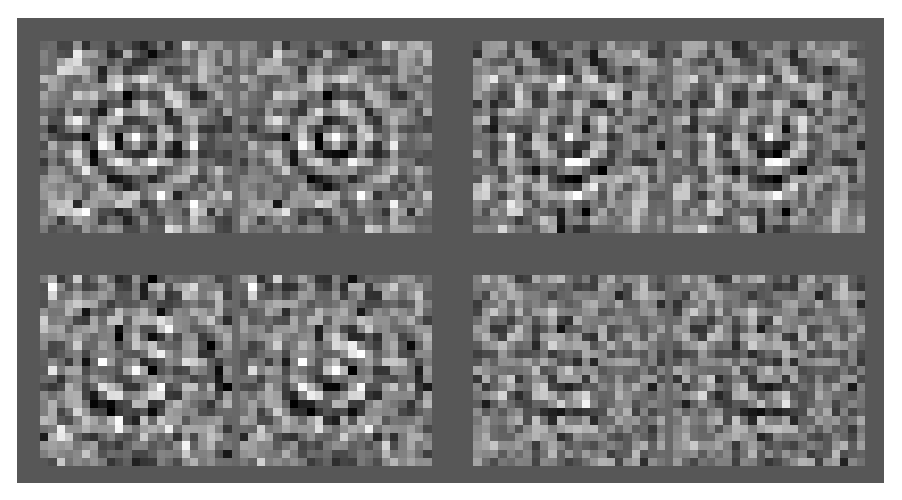
\includegraphics[width=0.5\textwidth, height=0.25\textwidth]{figures/deconv2.eps} 
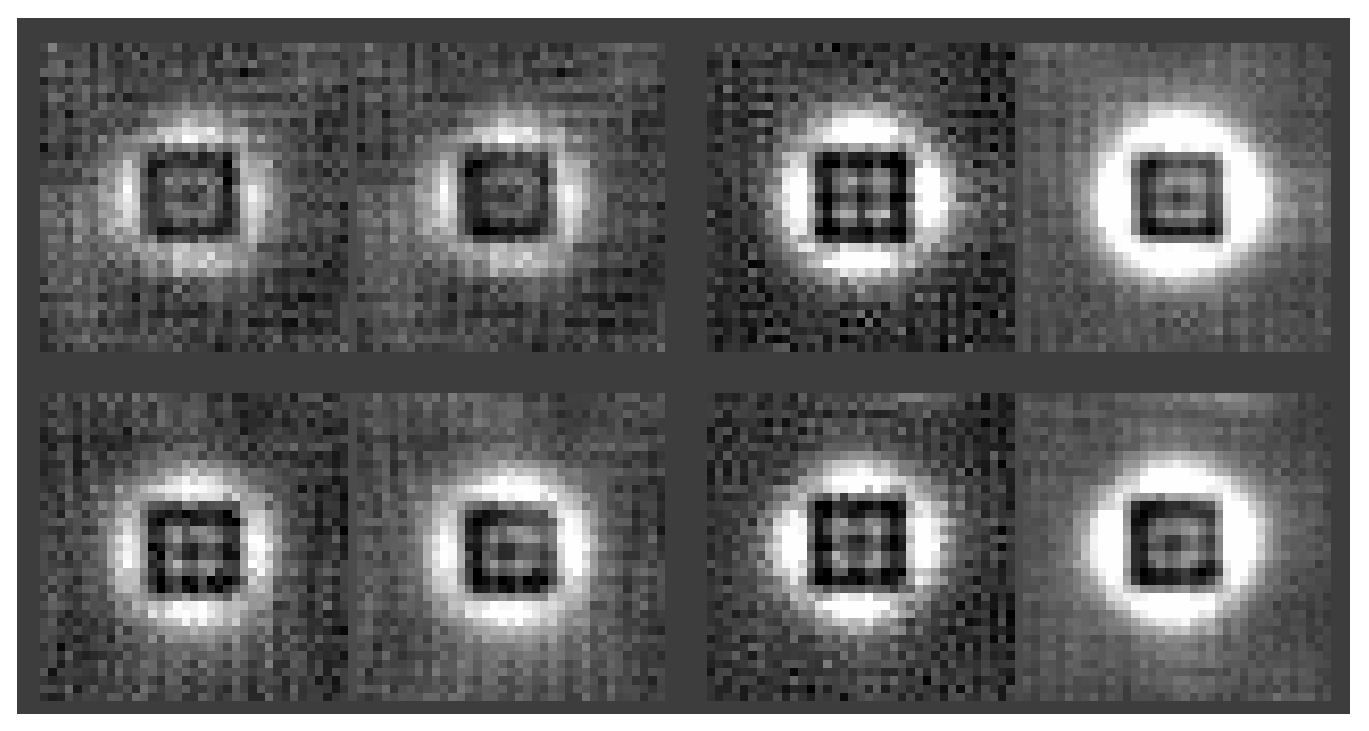
\includegraphics[width=0.5\textwidth, height=0.25\textwidth]{figures/size2.eps} \\
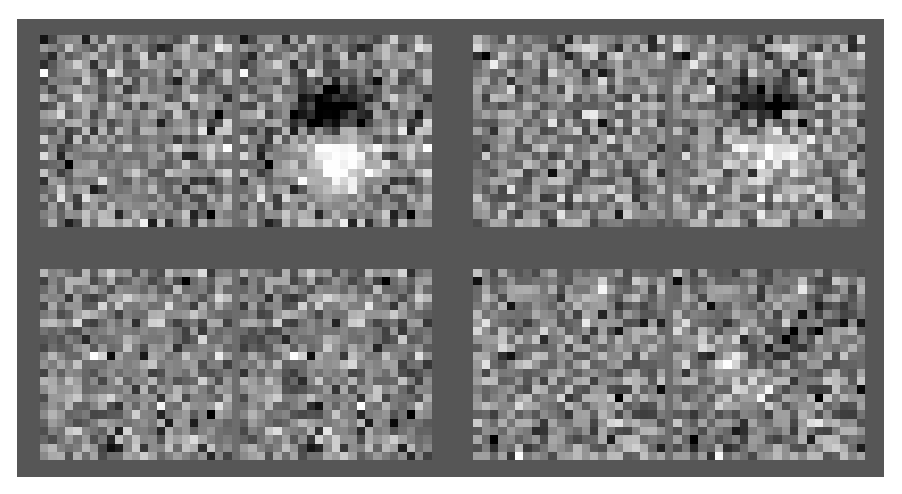
\includegraphics[width=0.5\textwidth, height=0.25\textwidth]{figures/order2.eps} 
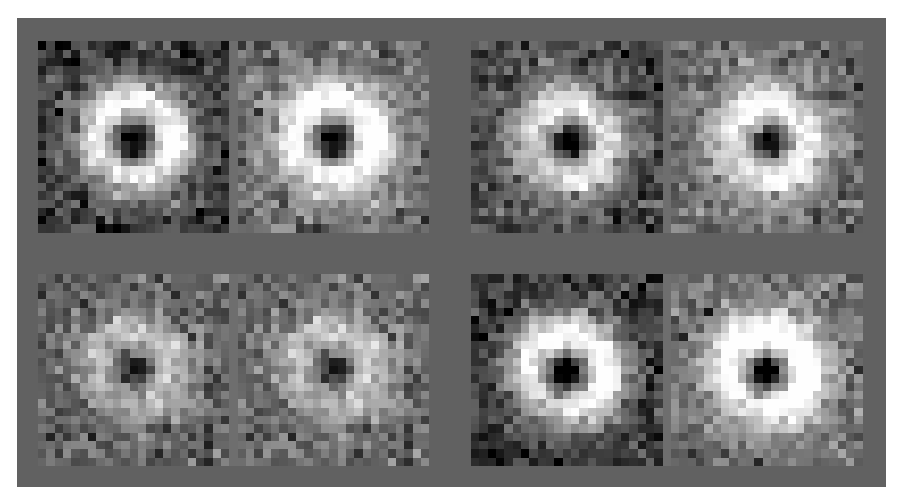
\includegraphics[width=0.5\textwidth, height=0.25\textwidth]{figures/shape2.eps} \\
\caption{Four example panels showing failure modes of the image
  subtraction software.  Each panel itself shows a 2x2 pair of
  difference images; on the {\it left} subpanel is the residual from
  the LOCAL fitting, and on the {\it right} from the SPATIAL fitting.
  Starting in the upper left and going clockwise, the first panel
  shows the residuals when deconvolving the template image; the
  ringing is characteristic of the deconvolution process.  Next, a set
  of difference images where the kernel dimensions (kernelSize) are
  too small to match the sources, leaving square kernel--sized
  residuals around each object.  Next, a set of images where the
  kernel shape (sigGauss) is inappropriate to match the sources; note
  that the LOCAL residuals show circular residuals, indicating the
  basis set itself is at fault (as opposed to the spatial model).
  Finally, in the lower--left, a set of images that demonstrate how
  the residuals degrade when the spatial kernel model is at fault.
  Note that the LOCAL residuals appear to be white noise, while the
  SPATIAL residuals show a clear dipole signature.  For this reason, a
  comparison between the LOCAL and SPATIAL residuals is a useful
  diagnostic of the spatial model.  }
\label{fig_galleryBad}
\end{figure}

\begin{figure}
\begin{center}
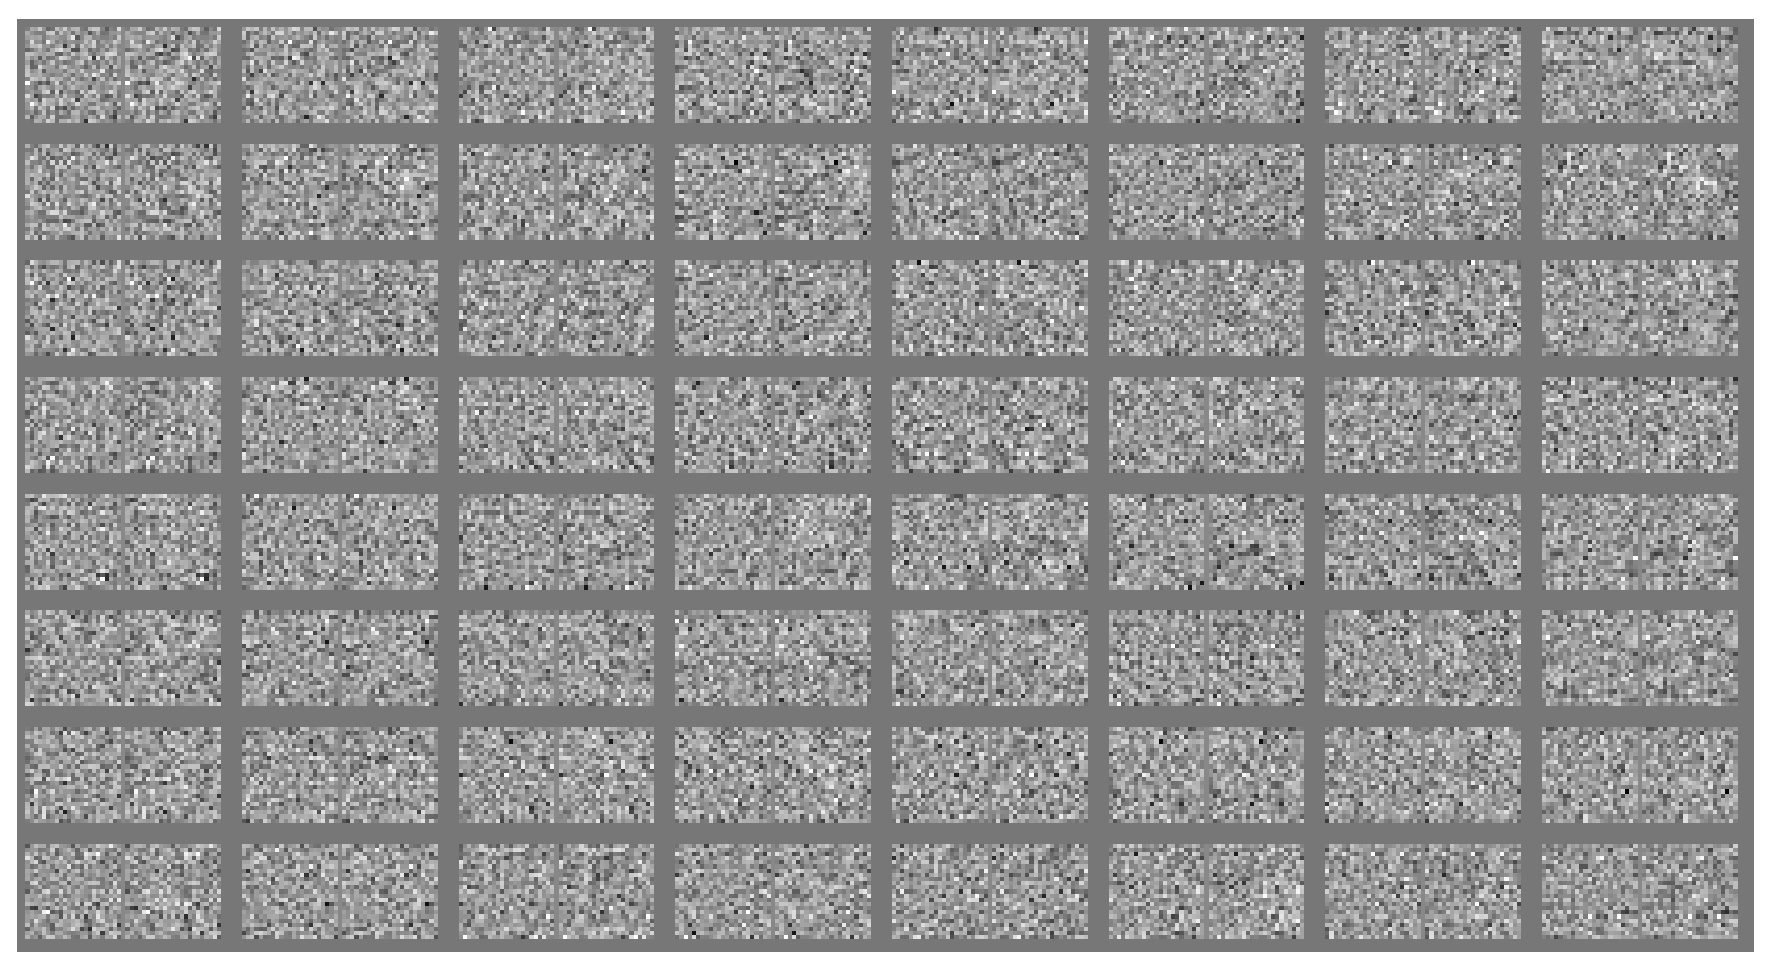
\includegraphics[width=0.9\textwidth]{figures/normal2.eps} \\
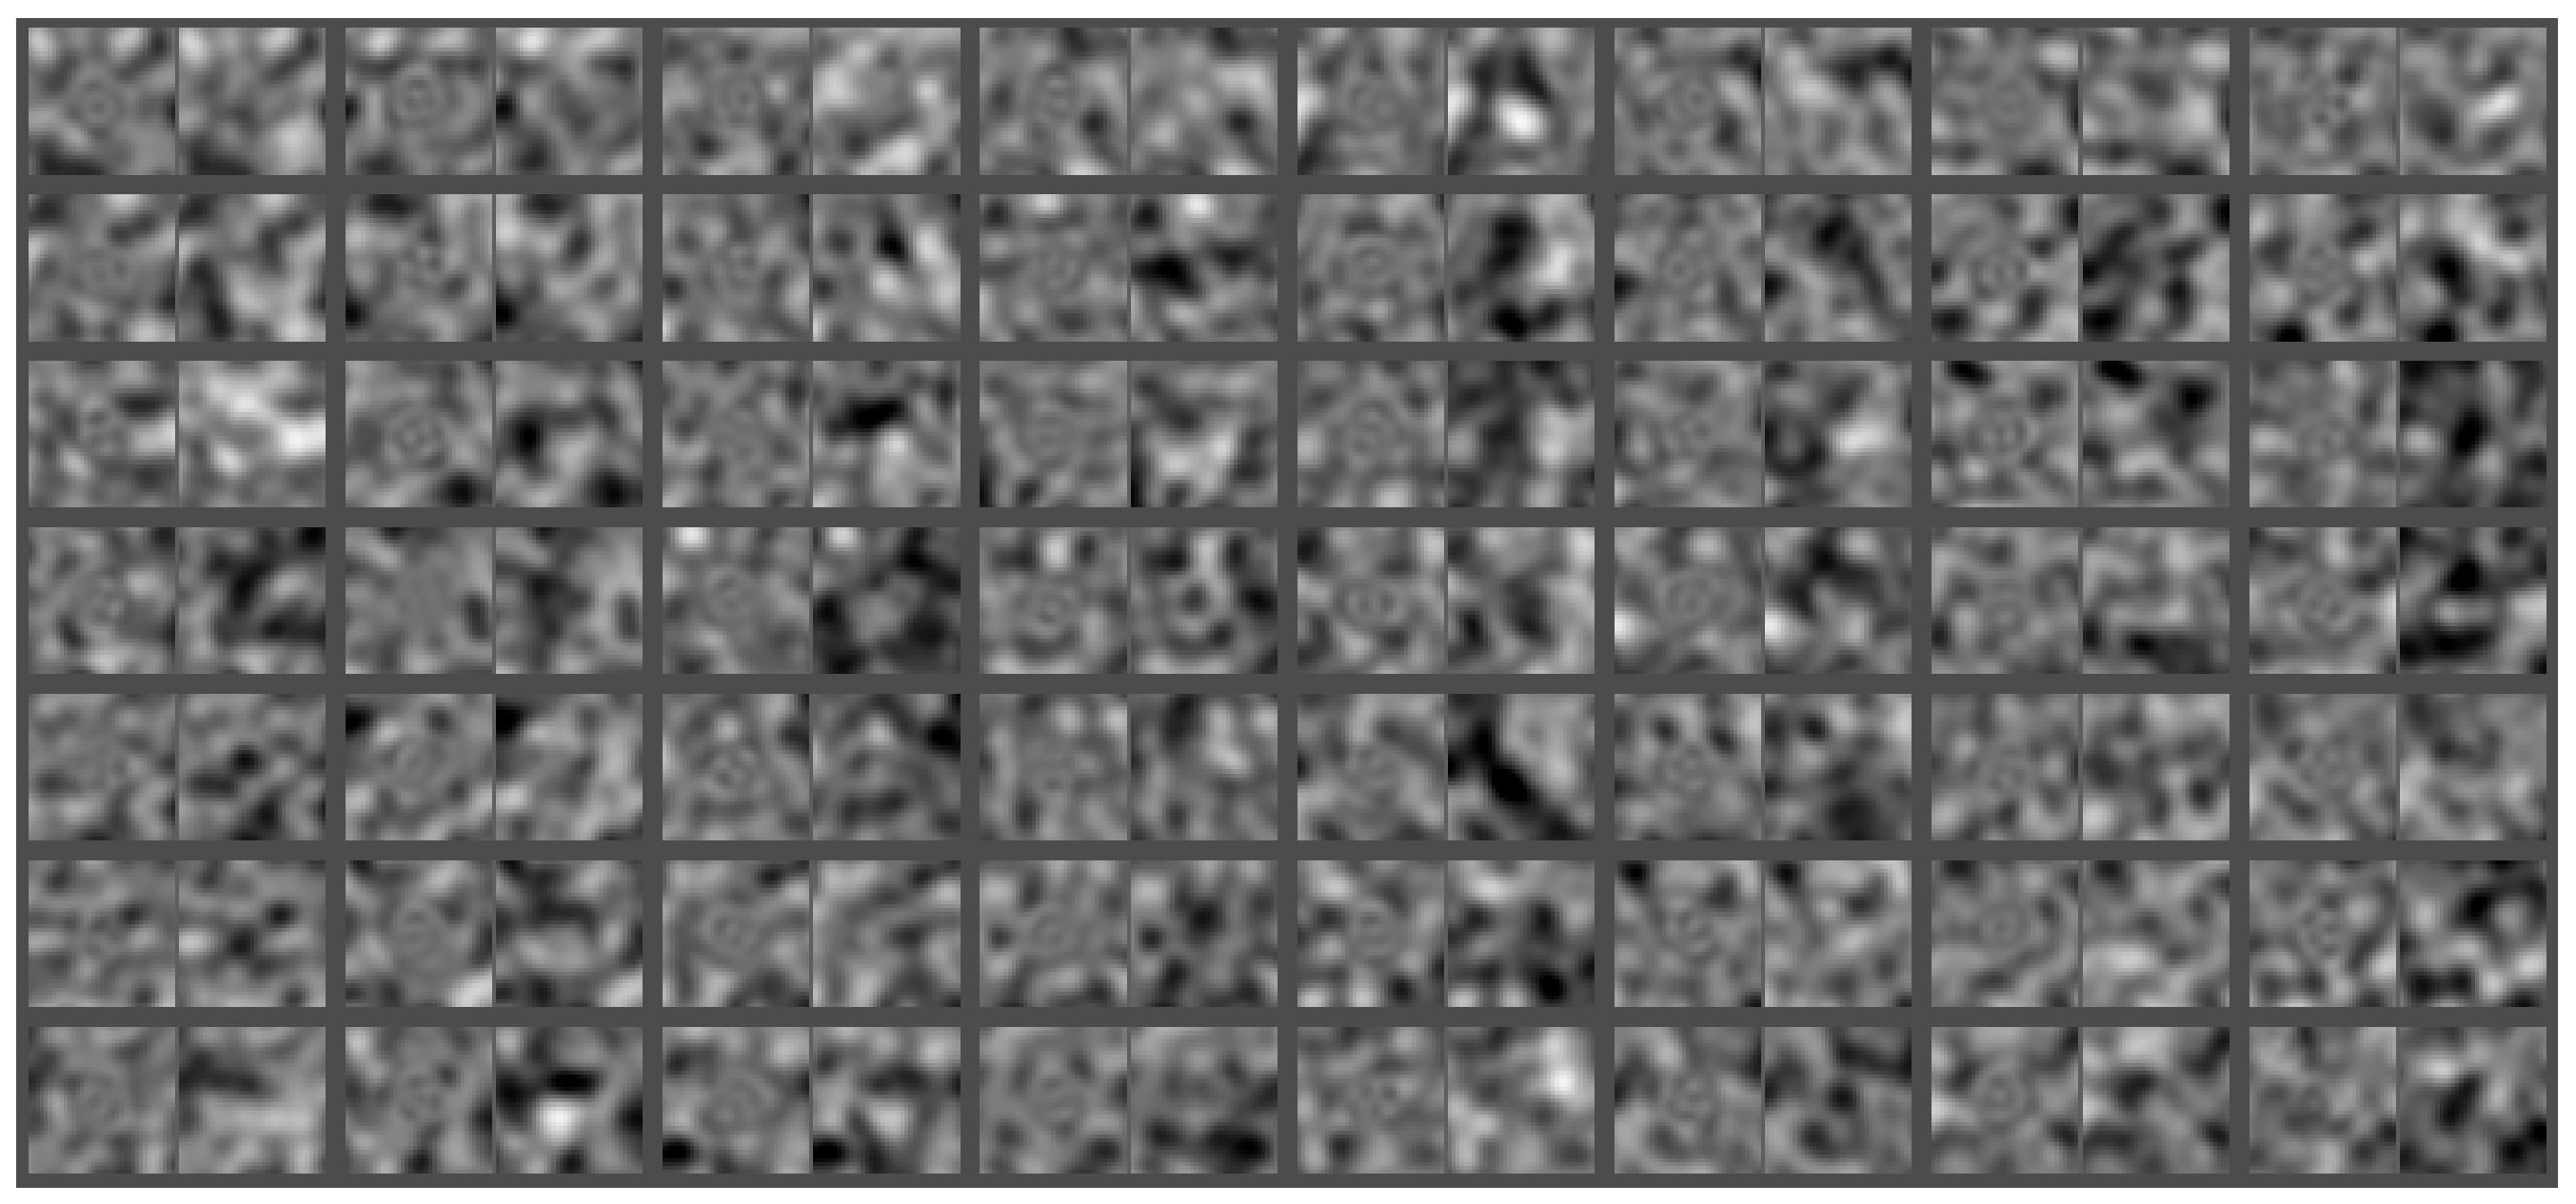
\includegraphics[width=0.9\textwidth]{figures/preconv2.eps} \\
\end{center}
\caption{Pairs of LOCAL,SPATIAL difference images in the case of
  successful image subtraction, similar to
  Figure~\ref{fig_galleryBad}.  The {\it top} set of data are from
  postfiltered analysis, while the {\it lower} set are from
  prefiltered data.  Note that the noise is smoother in the
  prefiltered data due to correlation with the PSF. }
\label{fig_galleryGood}
\end{figure}

\begin{figure}
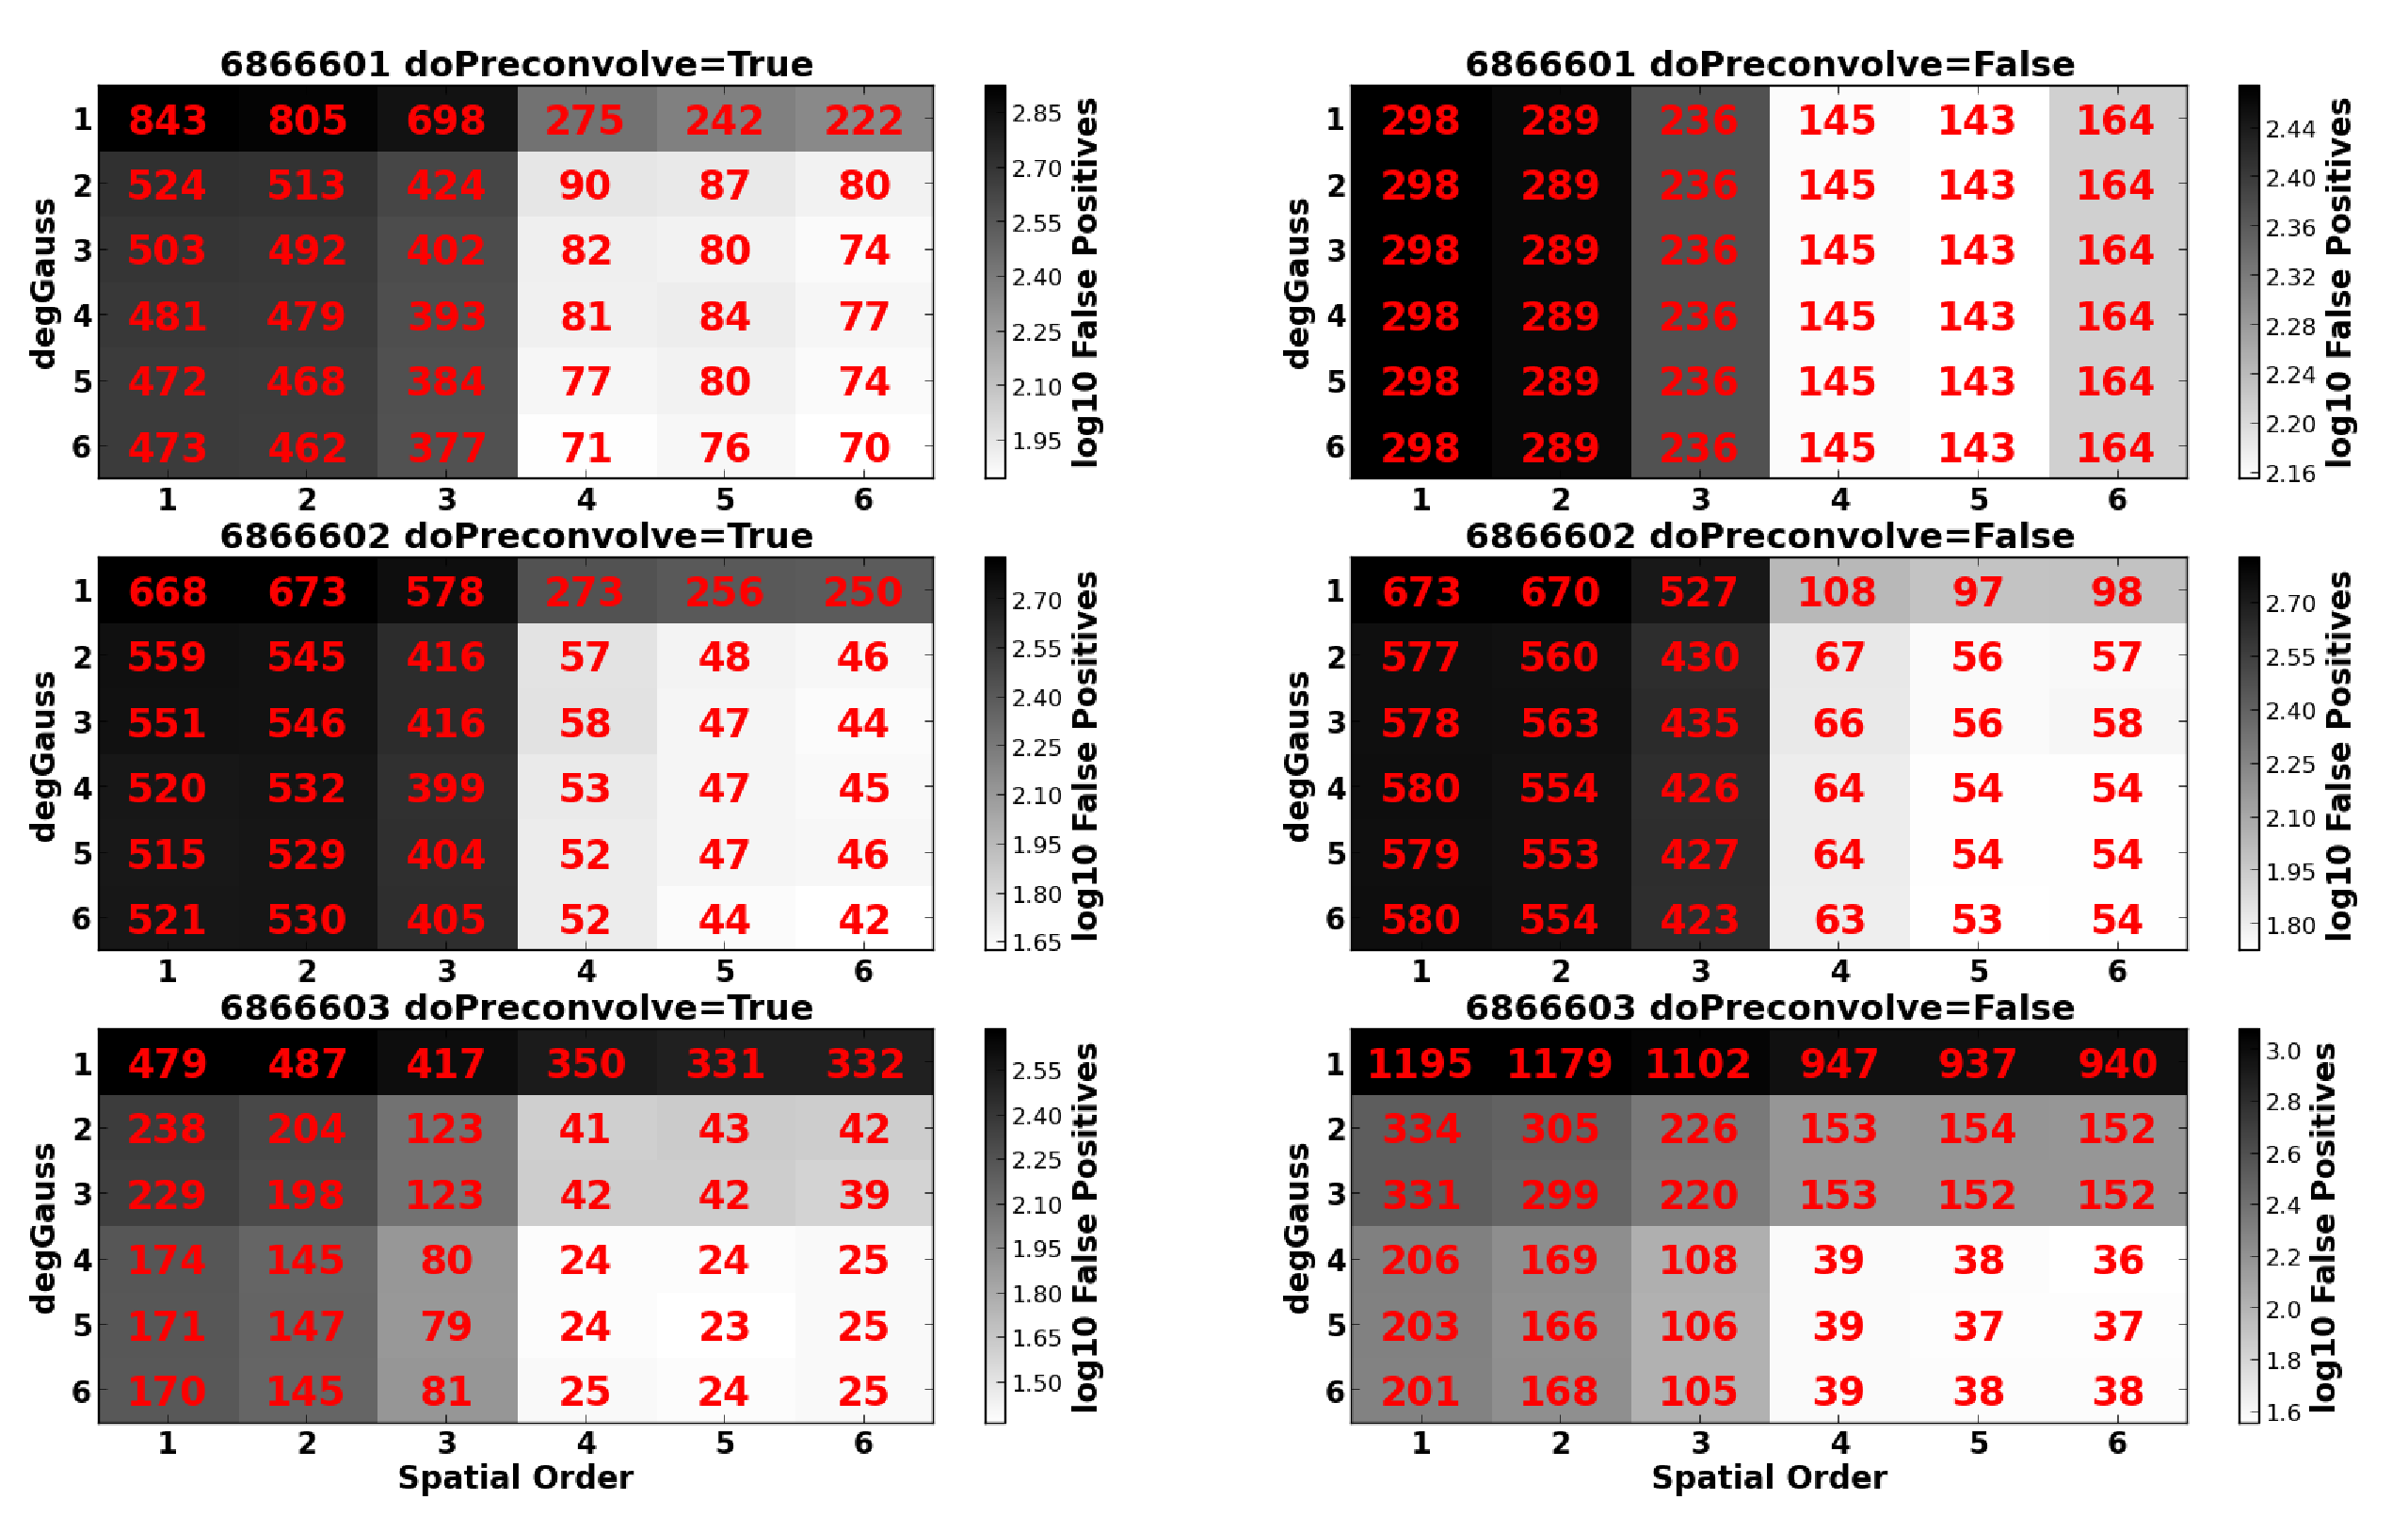
\includegraphics[width=1.0\textwidth]{figures/heatmap10.eps} \\
\caption{``Heat--map'' detailing the total numbers of 5--sigma false
  positives as a function of two main degrees of freedom: the maximum
  order of basis Laguerre polynomials along the y--axis, and the
  spatial order of the Chebyshev expansion of the spatial model along
  the x--axis.  The {\it left} column shows these results for
  prefiltering, while the {\it right} column shows this for the
  post--filtered analysis.  The best results listed in
  Table~\ref{tab-bestfp10}, with the associated configurations from
  Table~\ref{tab-bestconfig10}, correspond to the minimum in each of the
  subpanels.  }
\label{fp_heatmap}
\end{figure}

\begin{figure}
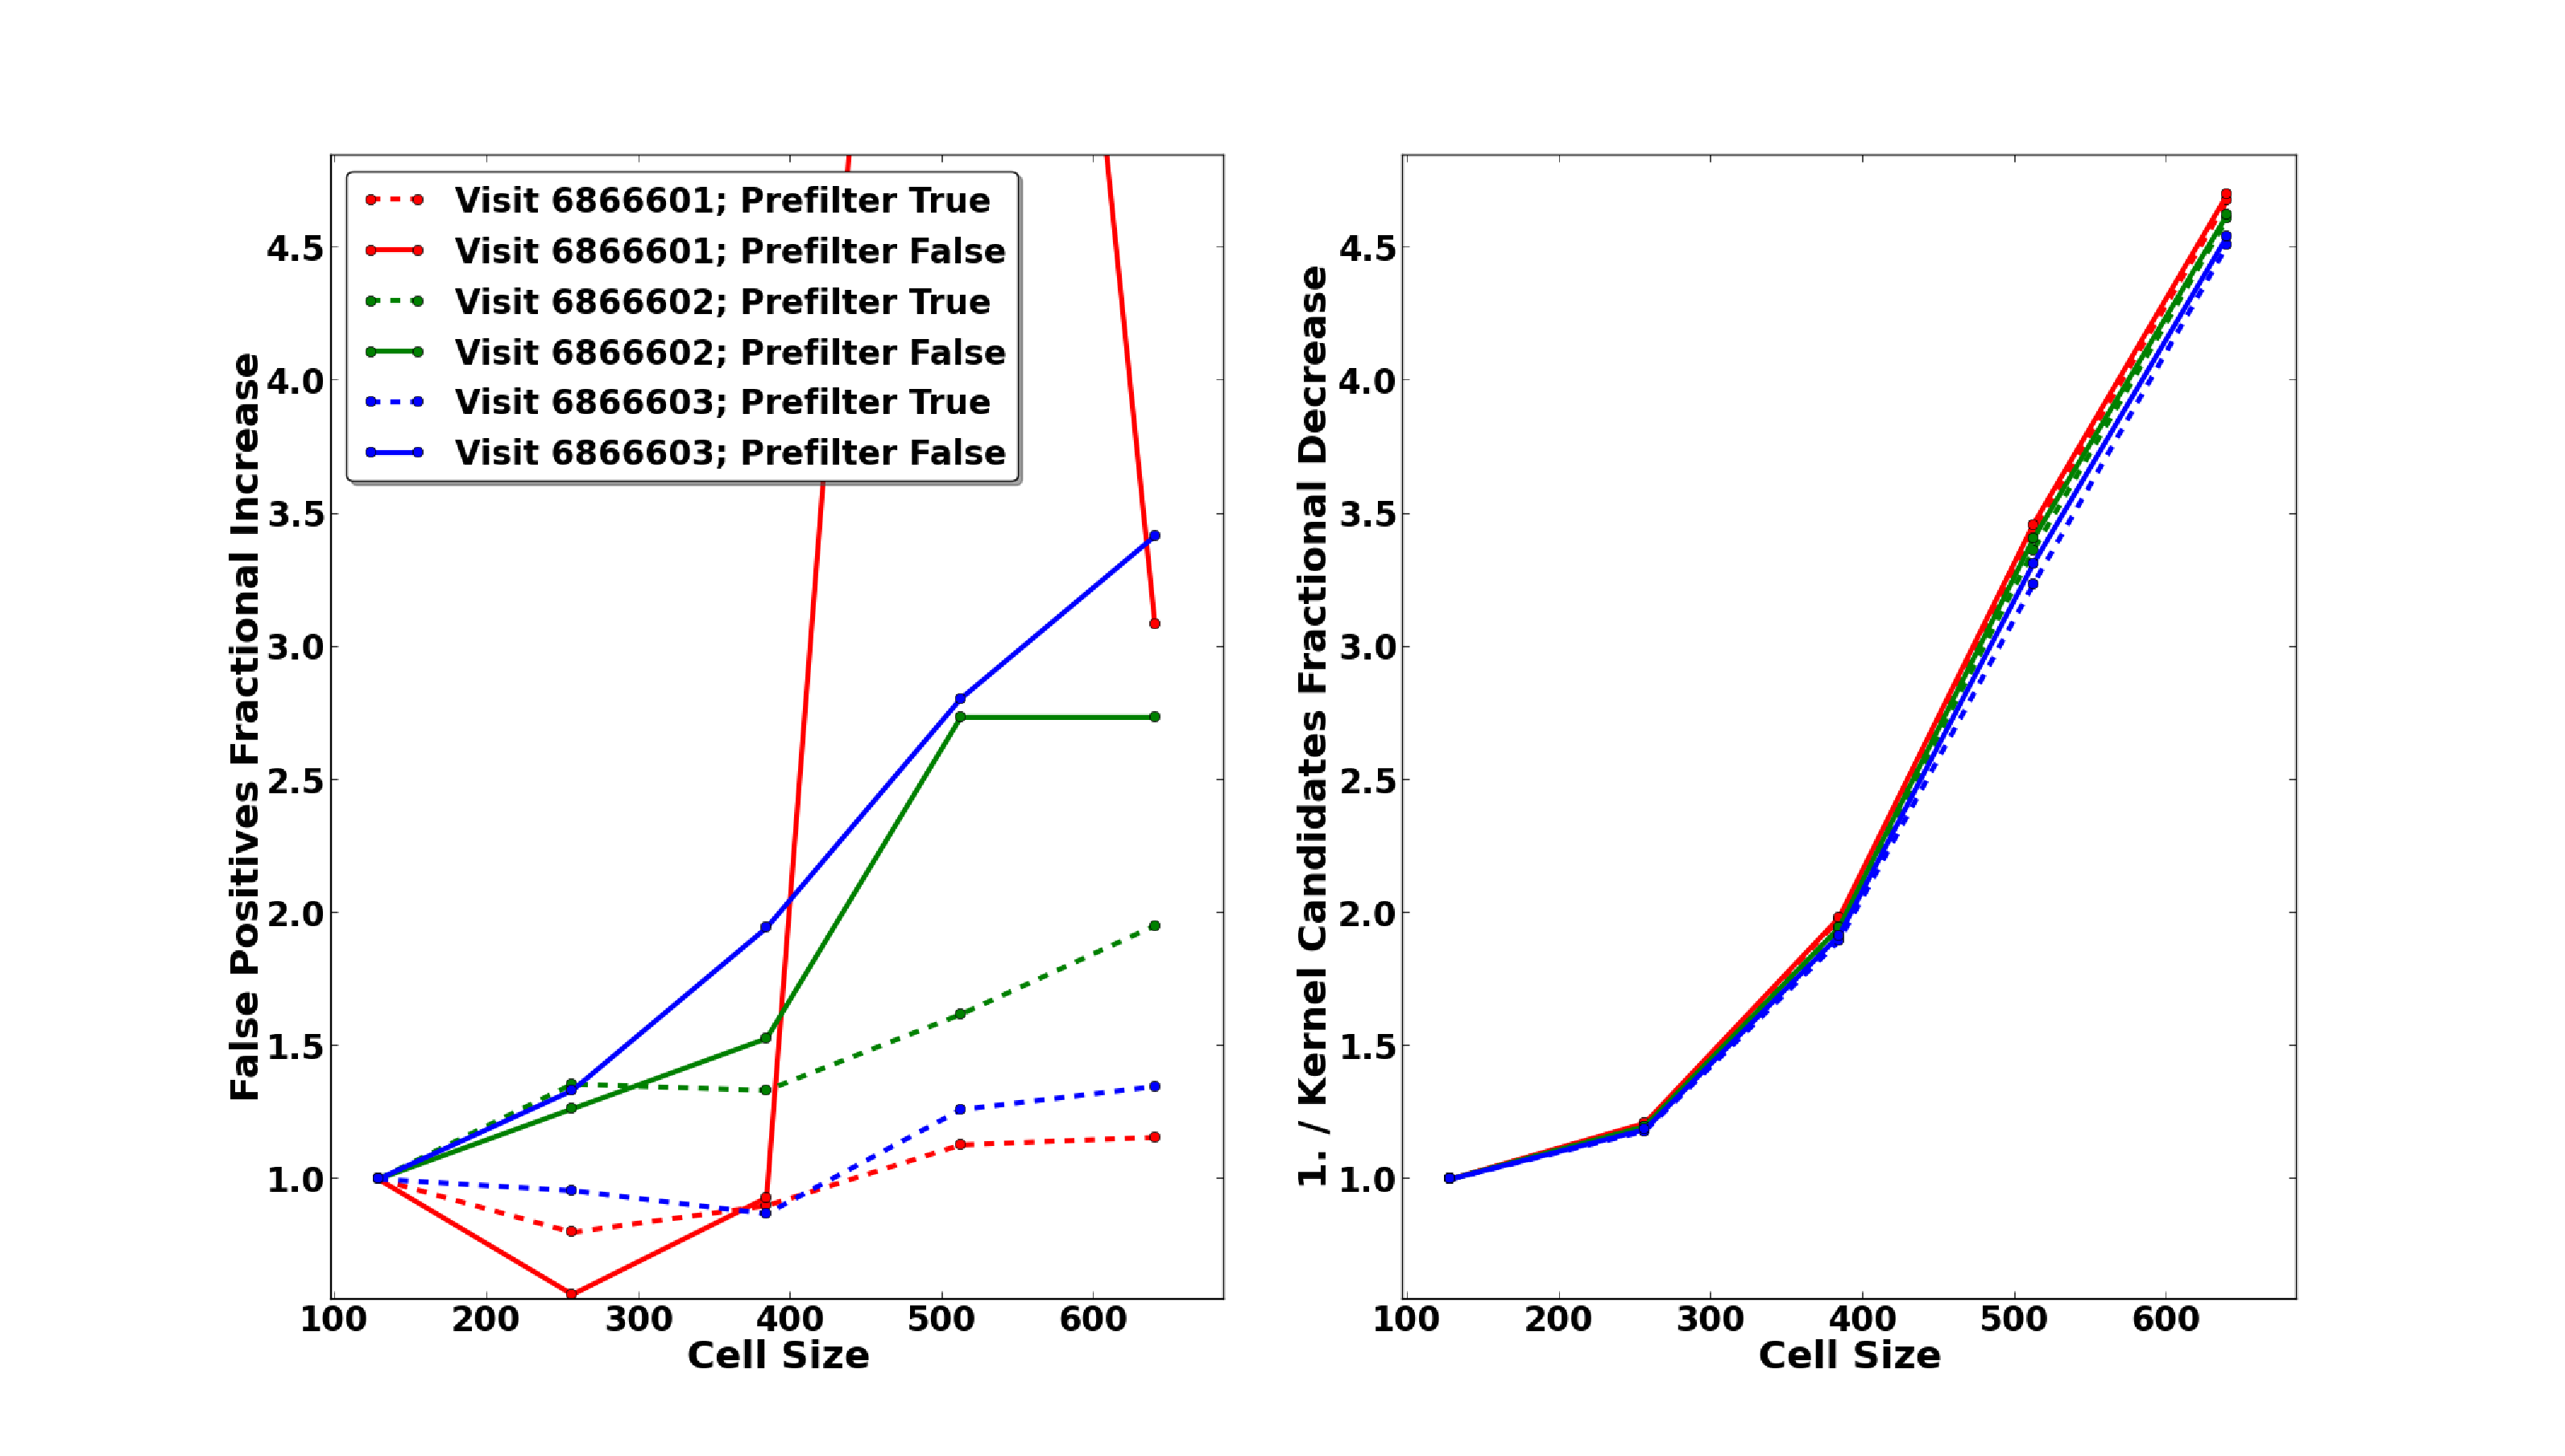
\includegraphics[width=1.0\textwidth]{figures/cellsize.eps} \\
\caption{False detections with cell size
}
\label{cellsize}
\end{figure}

\begin{figure}
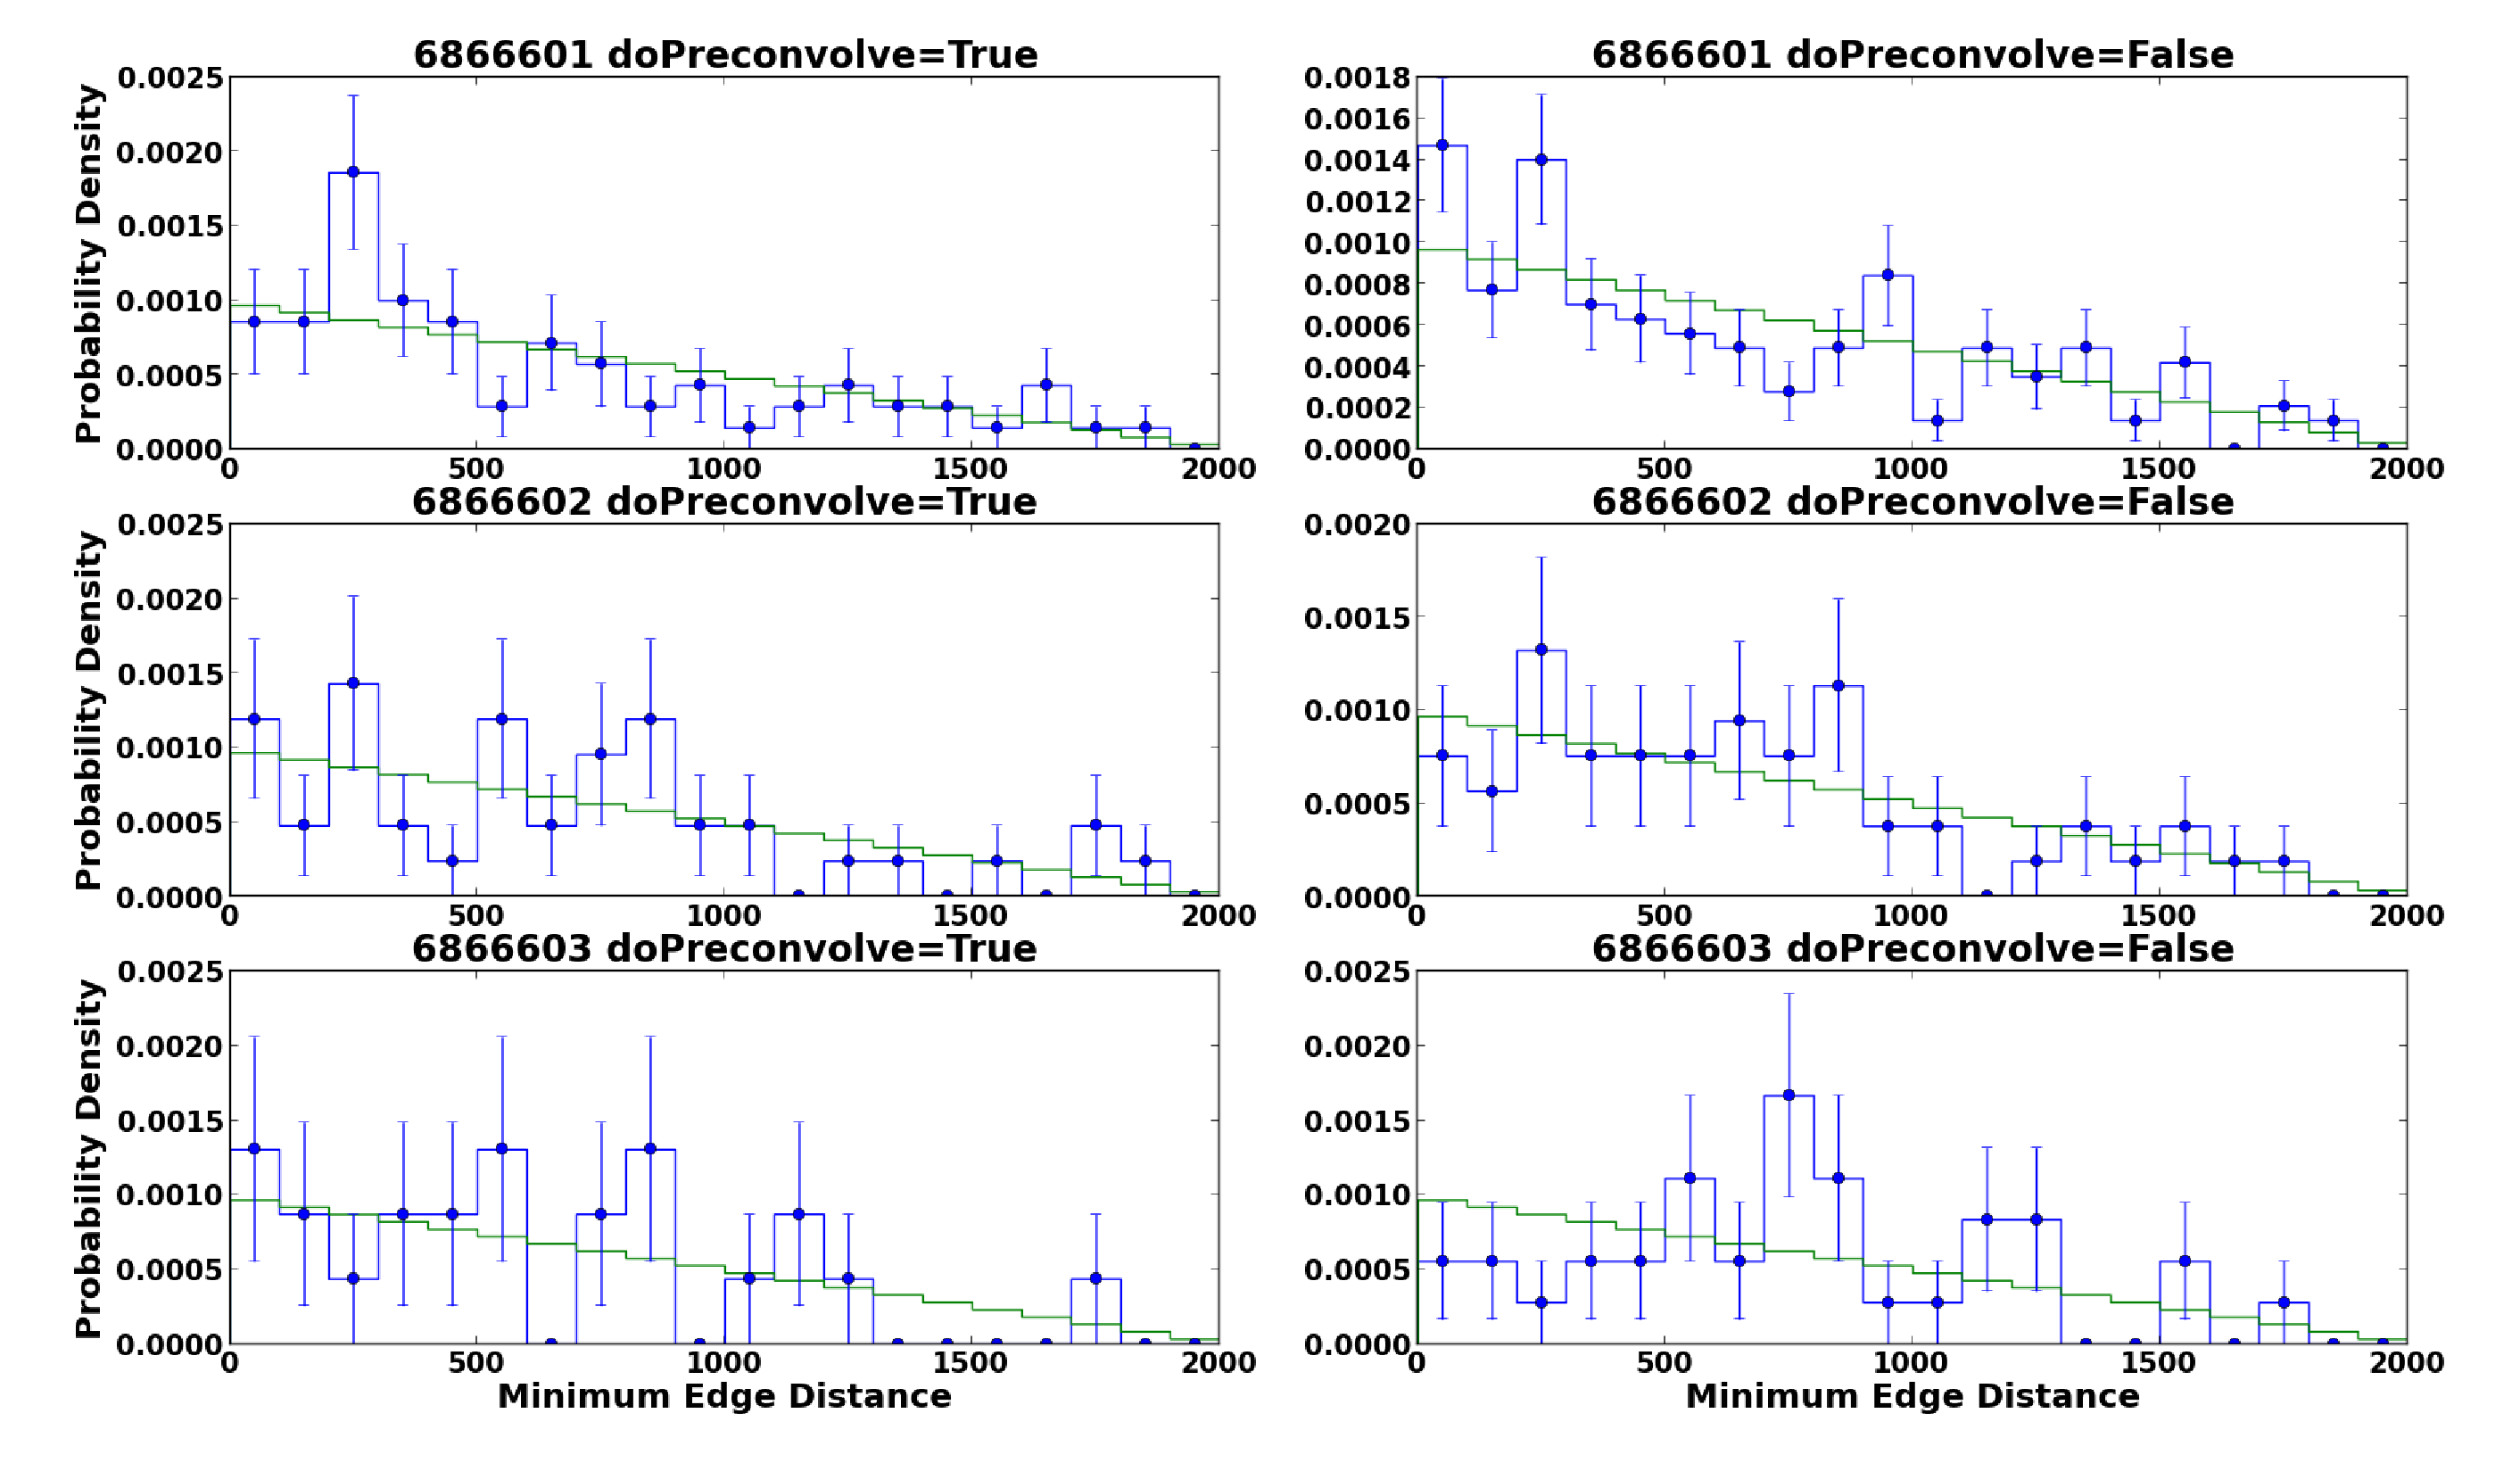
\includegraphics[width=1.0\textwidth]{figures/edge.eps} \\
\caption{Distribution of false detections as a function of the minimum
  distance from the edge of the sensor.  The {\it green} line shows
  the results from a random distribution of points.  The {\it blue}
  lines show the measured distributions, normalized as a probability
  density ($\sum y~\Delta x = 1$).  Error bars come from the square
  root of the number of points in each bin. }
\label{edgedist}
\end{figure}


\begin{figure}
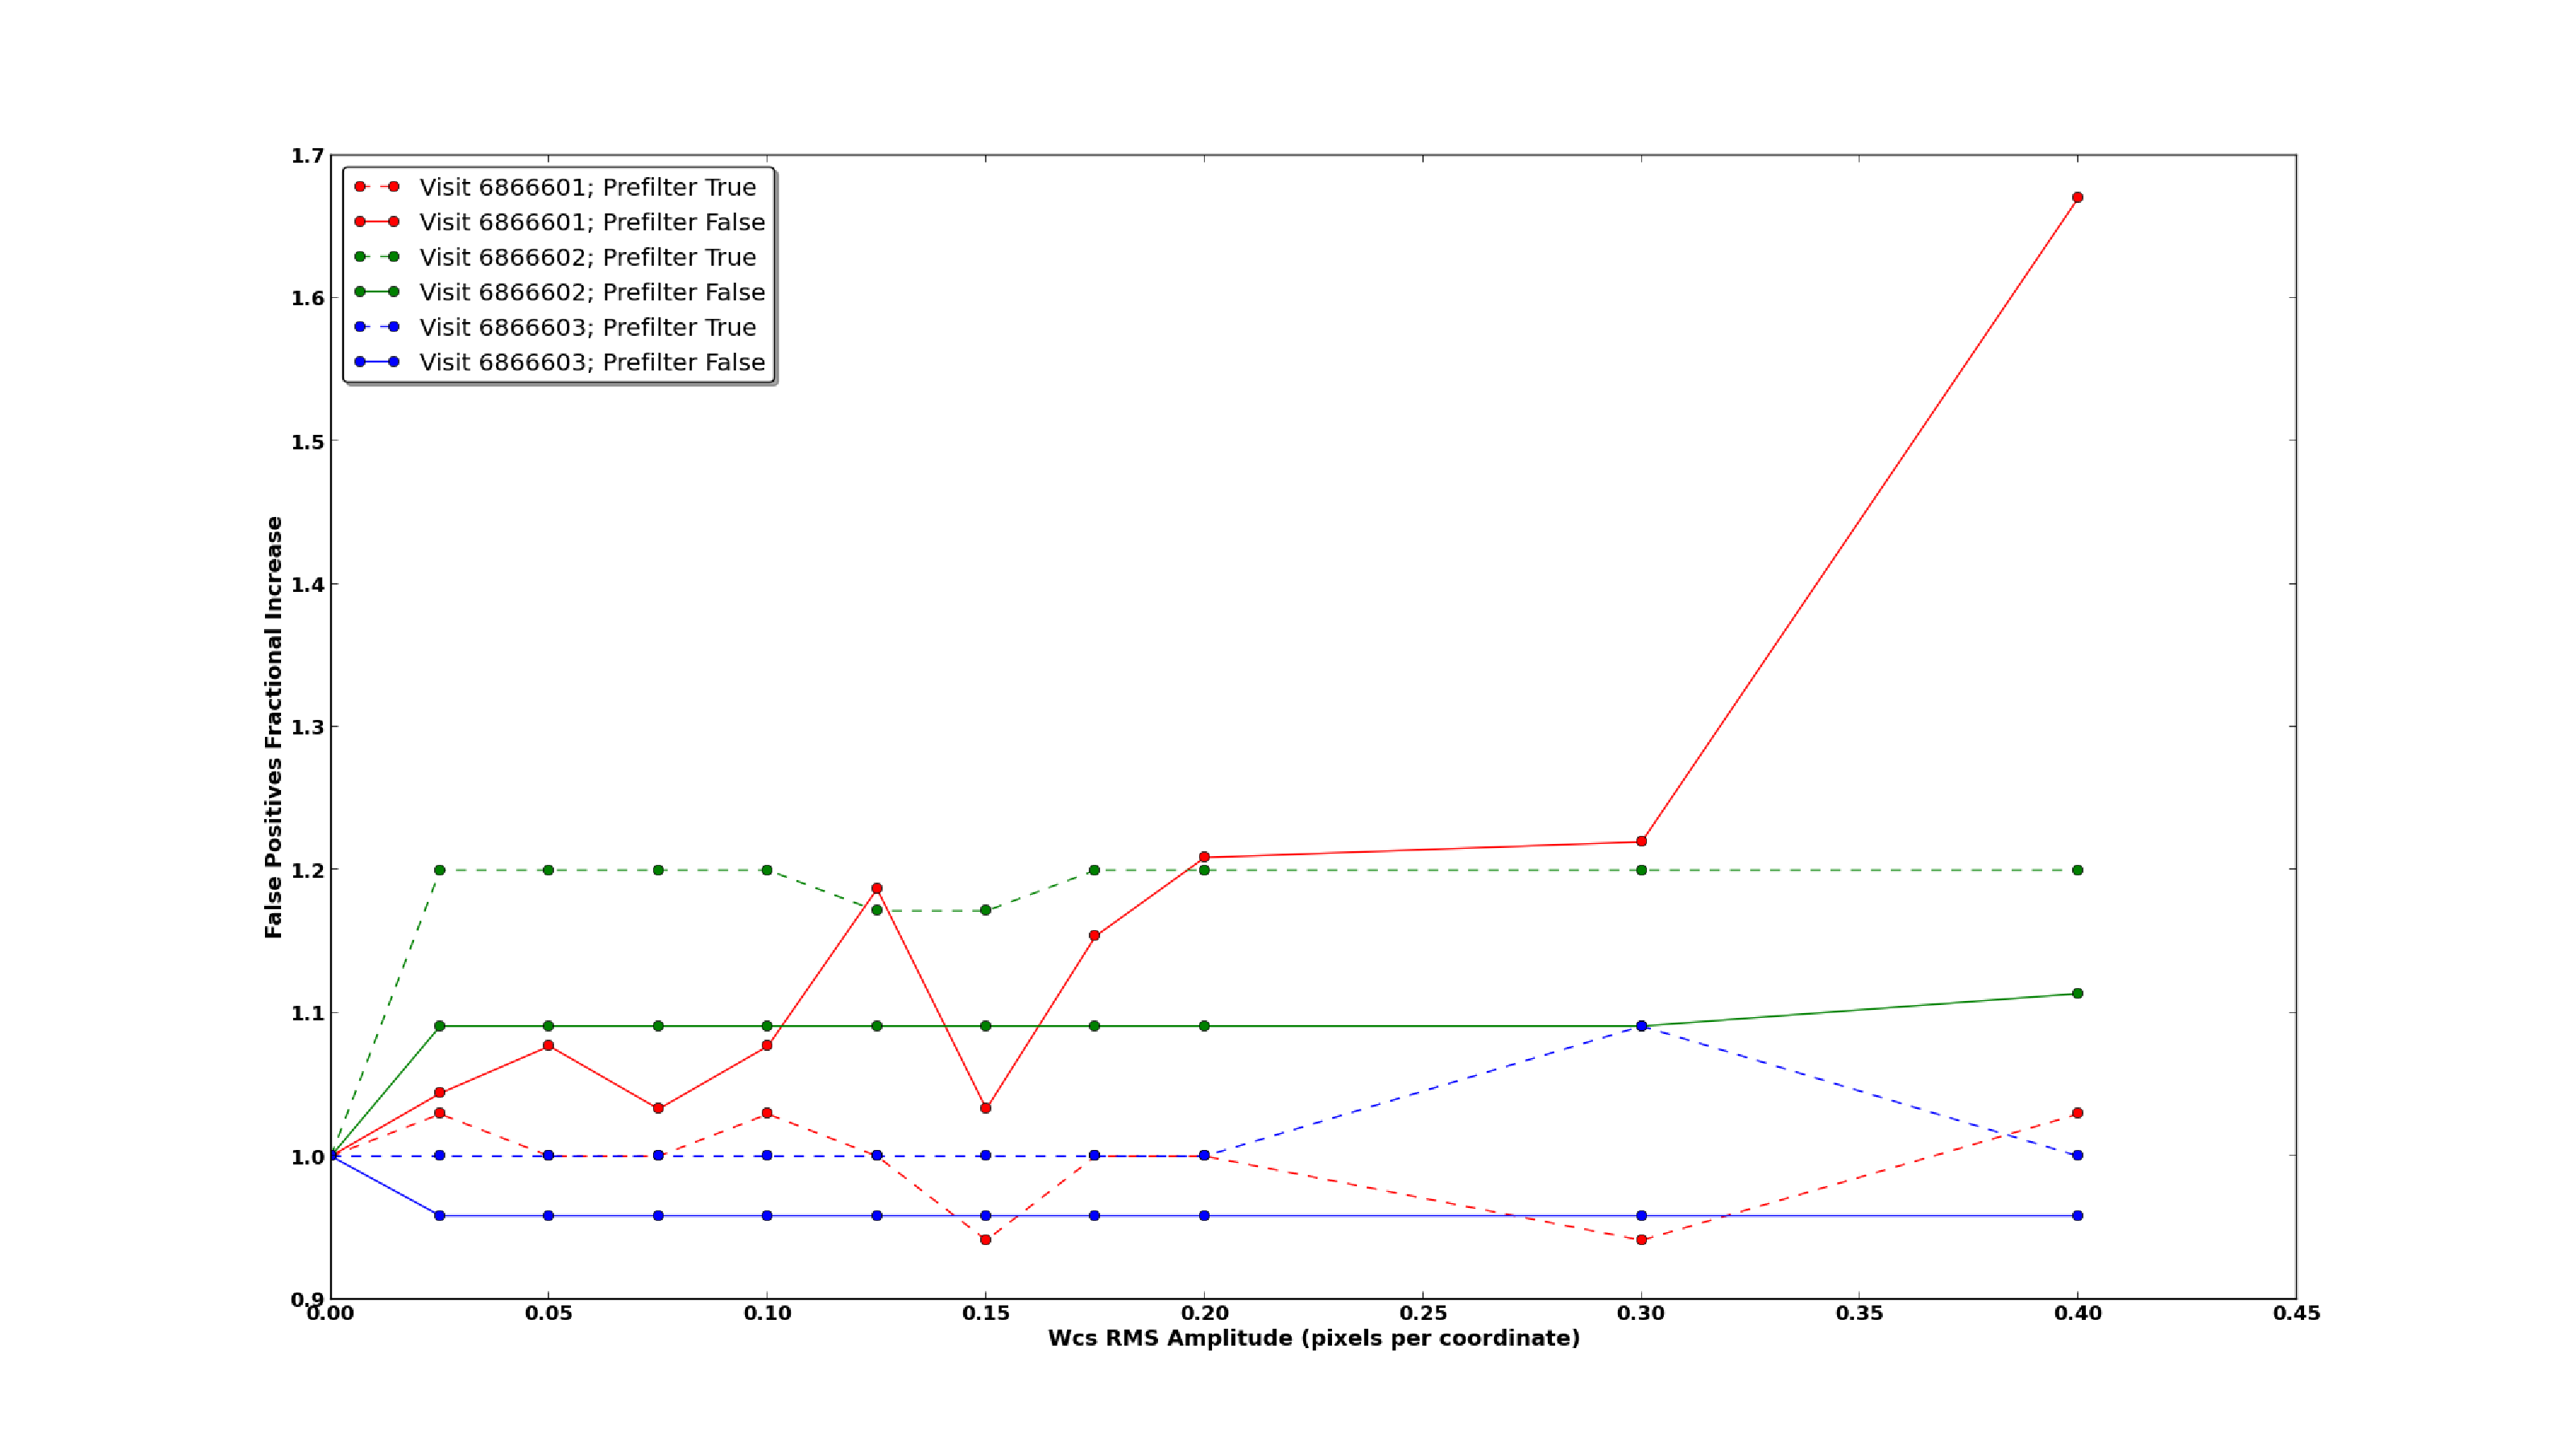
\includegraphics[width=1.0\textwidth]{figures/wcs_rms.eps} \\
\caption{Fractional increase in false detections as a function of the
  amplitude of random astrometric offsets added to the coordinates of
  sources before image-to-image registration.  The {\it red}, {\it
    green}, and {\it blue} lines correspond to visits v6866601,
  v6866602, and v6866603 respectively, while the {\it dashed} and {\it
    solid} lines correspond to prefiltering and postfiltering,
  respectively.}
\label{wcsrms}
\end{figure}

\begin{figure}
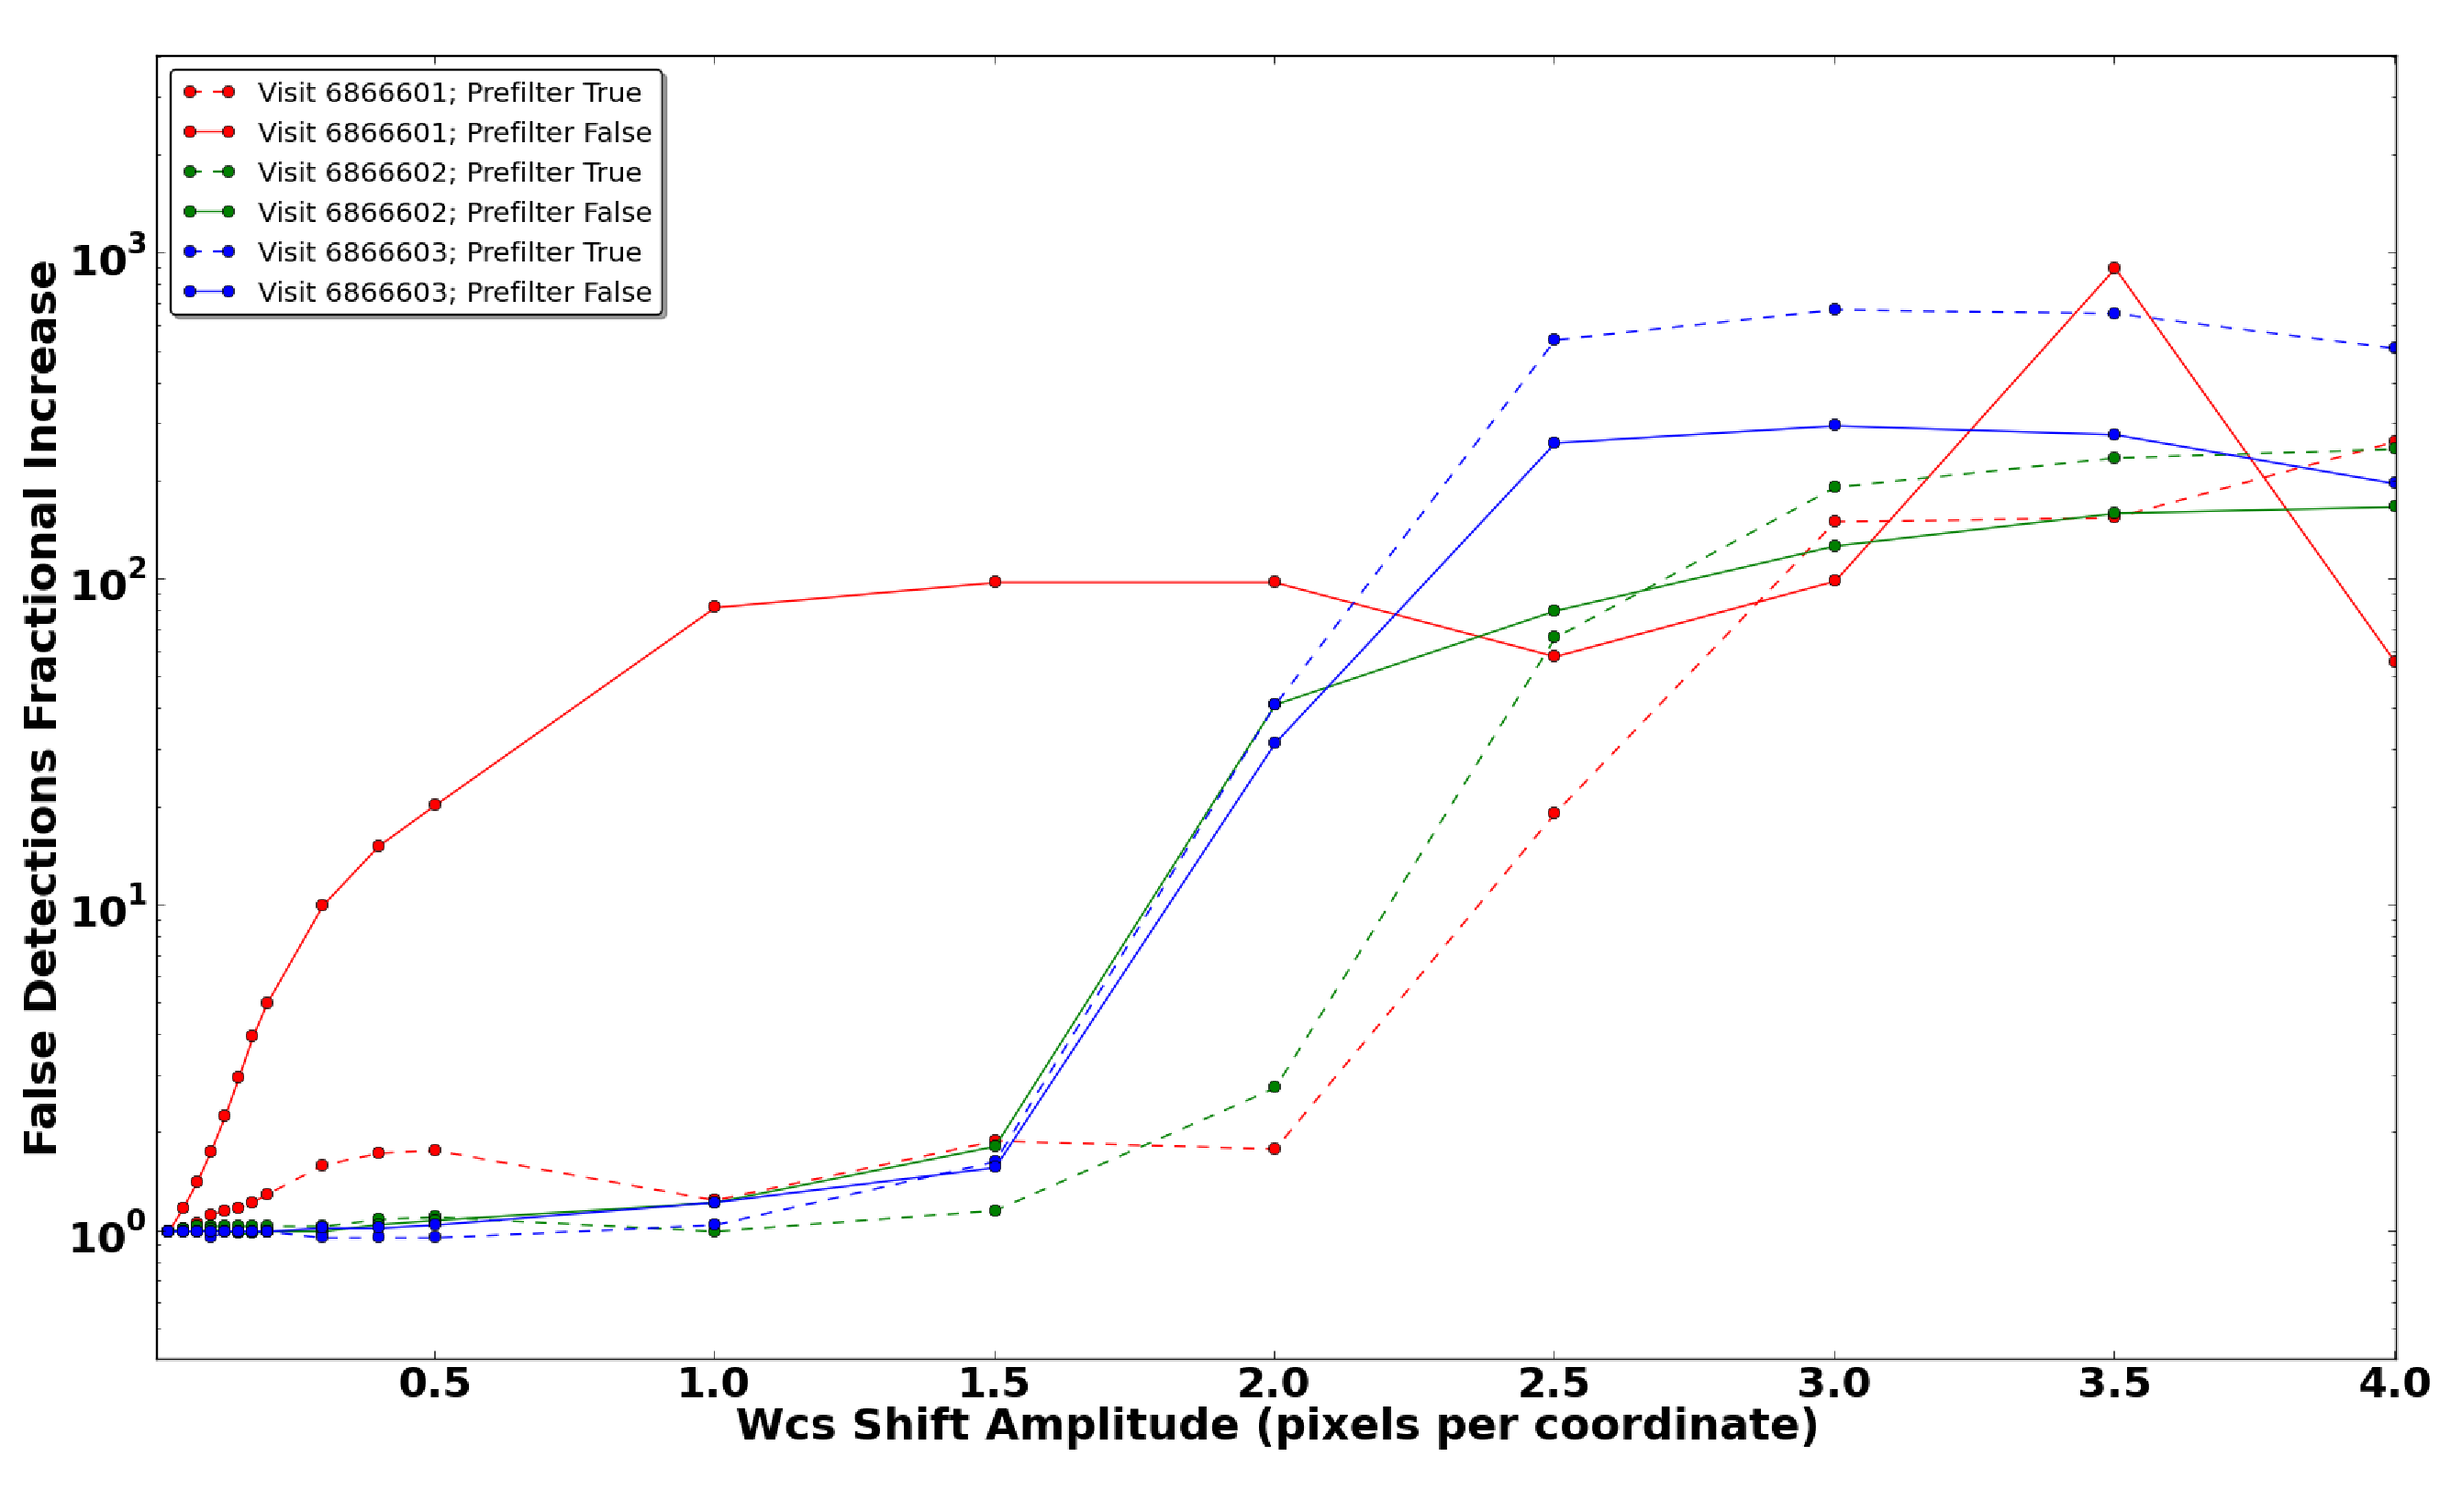
\includegraphics[width=1.0\textwidth]{figures/wcs_shift.eps} \\
\caption{Fractional increase in false detections as a function of bulk
  astrometric offsets added to the coordinates of sources before
  image-to-image registration.  The {\it red}, {\it green}, and {\it
    blue} lines correspond to visits v6866601, v6866602, and v6866603
  respectively, while the {\it dashed} and {\it solid} lines
  correspond to prefiltering and postfiltering, respectively.}
\label{wcsshift}
\end{figure}

\begin{figure}
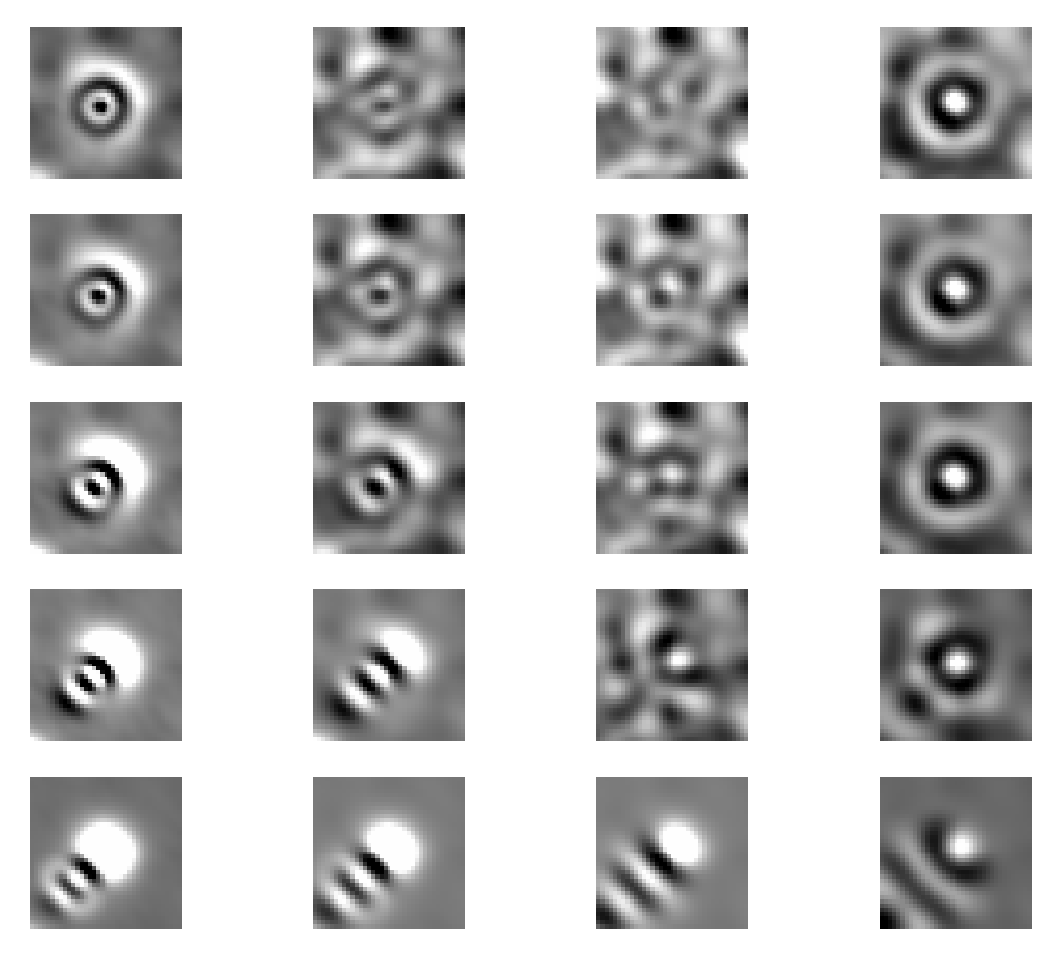
\includegraphics[width=0.8\textwidth]{figures/shift.eps} \\
\caption{Figure illustrating the ability of the kernel basis to
  compensate, locally, for the effects of misregistration.  Each
  element of the grid shows a single {\tt KernelCandidate} local
  difference image (visit=6866603, doPreFilter=True).  Columns
  indicate the Gaussian sigma of the basis, which is designed to have
  one Gaussian with the prescribed width, modified to fourth order.
  Rows indicate the amplitude of the astrometric offset that was
  introduced into the Source positions before image-to-image
  registration.  In the {\it top} row, we see that even with a small
  astrometric offset, the sigma=2 basis is unable to produce a quality
  subtraction, because the width is inappropriate for matching the two
  input PSFs (the theoretical Gaussian sigma here is 3.4 pixels).  At
  sigma=4 the basis is able to produce a quality subtraction, and by
  sigma=5 the basis is too large to match the PSFs.  In {\it row 4},
  we show that even for an astrometric offset of 4 pixels (0.8''), the
  sigma=4 basis can produce a reasonable difference image without
  structured residuals.  However, by {\it row 5}, with an offset of 6
  pixels, none of the Gaussians provide a successful local difference
  image.  The ability of the basis to compensate for bulk astrometric
  offsets is a function of the kernel width, and the kernel width is
  itself a function of the two input PSF FWHMs.  Thus there is a
  complicated dependence of the ability of the kernel to shift the
  centroids of stars.  Roughly, in our implementation, the basis may
  compensate for local astrometric residuals at a scale up to $\beta
  \times \sqrt{\sigma_S^2 - \sigma_T^2}$, which is the width of the
  largest Gaussian in our bases.}
\label{kernel_offsets}
\end{figure}


\end{document}
